%\usepackage{tcolorbox}
% Customizable fields and text areas start with % >> below.
% Lines starting with the comment character (%) are normally removed before release outside the collaboration, but not those comments ending lines

% svn info. These are modified by svn at checkout time.
% The last version of these macros found before the maketitle will be the one on the front page,
% so only the main file is tracked.
% Do not edit by hand!
\RCS$Revision: 302527 $
\RCS$HeadURL: svn+ssh://svn.cern.ch/reps/tdr2/notes/SUS-14-022/trunk/SUS-14-022.tex $
\RCS$Id: SUS-14-022.tex 302527 2015-09-03 20:04:06Z claudioc $
%%%%%%%%%%%%% local definitions %%%%%%%%%%%%%%%%%%%%%
% This allows for switching between one column and two column (cms@external) layouts
% The widths should  be modified for your particular figures. You'll need additional copies if you have more than one standard figure size.
\newcommand{\invfb}{\ensuremath{\,\rm{fb^{-1}}}\xspace}
\newcommand{\invpb}{\ensuremath{\,\rm{pb^{-1}}}\xspace}
\newcommand{\mt}{\ensuremath{\,{m_{\rm T}}}\xspace}
\newcommand{\mttwo}{\ensuremath{{M_{\rm T2}}}\xspace}
\newcommand{\mindphifour}{\ensuremath{\,{\Delta\phi_{\rm min}}}\xspace}
\newcommand{\IL}{\ensuremath{19.6\,\rm{fb^{-1}}}\xspace}
\newcommand{\SumMT}{ \ensuremath{\Sigma m_{\rm T}^{\tau_i}}\xspace}
\newcommand{\hadtau}{\ensuremath{\tau_{\rm had}}\xspace}
\newcommand{\Tau}{\ensuremath{\tau_{\rm had}}\xspace}
\newcommand{\tauMT}{\ensuremath{\,m_{\rm T}^{\hadtau}}\xspace}
\newcommand{\tauTau}{\ensuremath{\,\hadtau\hadtau}\xspace}
\newcommand{\muTau}{\ensuremath{\,\mu\hadtau}\xspace}
\newcommand{\eTau}{\ensuremath{\,e\hadtau}\xspace}
\newcommand{\leptonTau}{\ensuremath{\,\ell\hadtau}\xspace}
\newcommand{\chione}{\ensuremath{\widetilde{\chi}^{\pm}_1}\xspace}
\newcommand{\mvisi}{\ensuremath{m^{{\rm vis}(i)}}\xspace}
\newcommand{\etvisi}{\ensuremath{\et^{{\rm vis}(i)}}\xspace}
\newcommand{\vptvisi}{\ensuremath{\ptvec^{{\rm vis}(i)}}\xspace}
\newcommand{\PTslashvec}{\ensuremath{{\displaystyle{\not}\vec{p}}_{\rm T}}\xspace}
\newcommand{\neutralino}{\ensuremath{\tilde{\chi}^{0}_1}\xspace}
\newcommand{\met}{\ensuremath{\,{\ETslash}}\xspace}
\newcommand{\stau}{\ensuremath{\tilde{\tau}}\xspace}
\newcommand{\wjets}{\PW+jets}


\newlength\cmsFigWidth
\ifthenelse{\boolean{cms@external}}{\setlength\cmsFigWidth{0.85\columnwidth}}{\setlength\cmsFigWidth{0.4\textwidth}}
\ifthenelse{\boolean{cms@external}}{\providecommand{\cmsLeft}{top\xspace}}{\providecommand{\cmsLeft}{left\xspace}}
\ifthenelse{\boolean{cms@external}}{\providecommand{\cmsRight}{bottom\xspace}}{\providecommand{\cmsRight}{right\xspace}}
%%%%%%%%%%%%%%%  Title page %%%%%%%%%%%%%%%%%%%%%%%%
\cmsNoteHeader{SUS-14-022} % This is over-written in the CMS environment: useful as preprint no. for export versions
% >> Title: please make sure that the non-TeX equivalent is in PDFTitle below
\title{Search for electroweak production of charginos in final states with two tau leptons in pp collisions at $\sqrt{s}= 8$\TeV}

% >> Authors
%Author is always "The CMS Collaboration" for PAS and papers, so author, etc, below will be ignored in those cases
%For multiple affiliations, create an address entry for the combination
%To mark authors as primary, use the \author* form
\address[neu]{Northeastern University}
\address[fnal]{Fermilab}
\address[cern]{CERN}
\author[cern]{The CMS Collaboration}


% >> Date
% The date is in yyyy/mm/dd format. Today has been
% redefined to match, but if the date needs to be fixed, please write it in this fashion.
% For papers and PAS, \today is taken as the date the head file (this one) was last modified according to svn: see the RCS Id string above.
% For the final version it is best to "touch" the head file to make sure it has the latest date.
\date{\today}

% >> Abstract
% Abstract processing:
% 1. **DO NOT use \include or \input** to include the abstract: our abstract extractor will not search through other files than this one.
% 2. **DO NOT use %**                  to comment out sections of the abstract: the extractor will still grab those lines (and they won't be comments any longer!).
% 3. For PASs: **DO NOT use tex macros**         in the abstract: CDS MathJax processor used on the abstract doesn't understand them _and_ will only look within $$. The abstracts for papers are hand formatted so macros are okay.
\abstract{
 A search for electroweak production of supersymmetric particles is performed 
with two tau leptons in the final state.
 These results are based on 18.1 to 19.6  fb$^{-1}$  of proton-proton collisions at $\sqrt{s}$ = 8\TeV
 collected with the CMS detector at the CERN Large Hadron Collider.
The observed events are found to be consistent with the standard model prediction. Upper limits are set on the masses of the lightest 
chargino and the lightest neutralino, assuming the third generation sleptons are the lightest sleptons and their masses are at a middle 
point between the chargino and the neutrralino. In the context of simplified model spectra, charginos lighter than 430\GeV are excluded 
at 95\% confidence level in the case of massless neutralino.
}    

% >> PDF Metadata
% Do not comment out the following hypersetup lines (metadata). They will disappear in NODRAFT mode and are needed by CDS.
% Also: make sure that the values of the metadata items are sensible and are in plain text:
% (1) no TeX! -- for \sqrt{s} use sqrt(s) -- this will show with extra quote marks in the draft version but is okay).
% (2) no %.
% (3) No curly braces {}.
\hypersetup{%
pdfauthor={IPM TauTau Group},%
pdftitle={Search for electroweak production of charginos in di-tau final states in pp collisions at sqrt(s)= 8 TeV with the CMS detector},%
pdfsubject={CMS},%
pdfkeywords={CMS, physics, software, computing}}

\maketitle %maketitle comes after all the front information has been supplied
% >> Text
%%%%%%%%%%%%%%%%%%%%%%%%%%%%%%%%  Begin text %%%%%%%%%%%%%%%%%%%%%%%%%%%%%
%% **DO NOT REMOVE THE BIBLIOGRAPHY** which is located before the appendix.
%% You can take the text between here and the bibiliography as an example which you should replace with the actual text of your document.
%% If you include other TeX files, be sure to use "\input{filename}" rather than "\input filename".
%% The latter works for you, but our parser looks for the braces and will break when uploading the document.
%%%%%%%%%%%%%%%
\section{Introduction}
\label{sect:introduction}
Supersymmetry \cite{Martin:1997ns} (SUSY) is one of the most promising extensions of the 
Standard Model of the elementary particles (SM) which solves both the 
quadratic divergencies and hierarchy problems simultaneously. It introduces a new symmetry between the bosons and fermions and 
for every particle an sparticle is defined which is exactly the same, but differ in spin by 1/2. 

In a hadron collider, like LHC, it is expected to see the signature of the colored SUSY partners, 
but the very extensive search in the LHC experiments pushes the mass of the colored particles much 
beyond the previous expectations. 
Looking at other sectors of the SUSY, e.g, electroweak production of the sparticles, is motivated not to miss SUSY in a corner. 
To cancel the quadratic divergency of the quantum corrections to higgs boson mass,  sleptons, charginos and neutralinos 
should not be heavier than few hundred \GeV \cite{1988NuPhB.306...63B, deCarlos:1993yy}. So they should be accessible by the current data.
A search for new physics using ~20 \fbinv of proton-proton collision data from CMS collected in 2012 in the center of mass energy of 
$\sqrt{s}$ = 8 \TeV  is documented in this report. 
Although the search is sensitive to any high scale new physics with a missing transverse momentum (\MET), 
an R-parity conserving SUSY model is used to illustrate the performance of the method.

Due to the special role of the third generation of the sparticles, events with two taus in the final state 
accompanying with the missing transverse energy (\met) are considered.
The two taus can be generated in the cascade of the staus or charginos:
\begin{linenomath}
\begin{equation}
p + p \rightarrow \tilde{\chi_{1}^{+}} + \tilde{\chi_{1}^{-}} ~~\mathrm{or}~~  p + p \rightarrow \tilde{\tau} + \tilde{\tau}
\end{equation}
\end{linenomath}
when 
\begin{linenomath}
\begin{equation}
\tilde{\chi_{1}^{+}} \rightarrow \tilde{\tau} + \nu ~~\mathrm{or}~~  \tilde{\chi_{1}^{+}} \rightarrow \tilde{\nu}_{\tau} + \tau 
\end{equation}
\end{linenomath}
and 
\begin{linenomath}
\begin{equation}
\tilde{\tau} \rightarrow \tau + \tilde{\chi_{1}^{0}} ~~\mathrm{or}~~  \tilde{\nu}_{\tau} \rightarrow \nu + \tilde{\chi_{1}^{0}} 
\end{equation}
\end{linenomath}
and $\tilde{\chi_{1}^{0}}$ can not be detected and appears as missing transverse momentum (\met).
In this note, we mainly focus on the $\tilde{\chi_{1}^{+}}\tilde{\chi_{1}^{-}}$ production which has a higher 
production cross section. Figure \ref{fig:Productions} shows our favorite decays.

\begin{figure}[!htb]
\centering
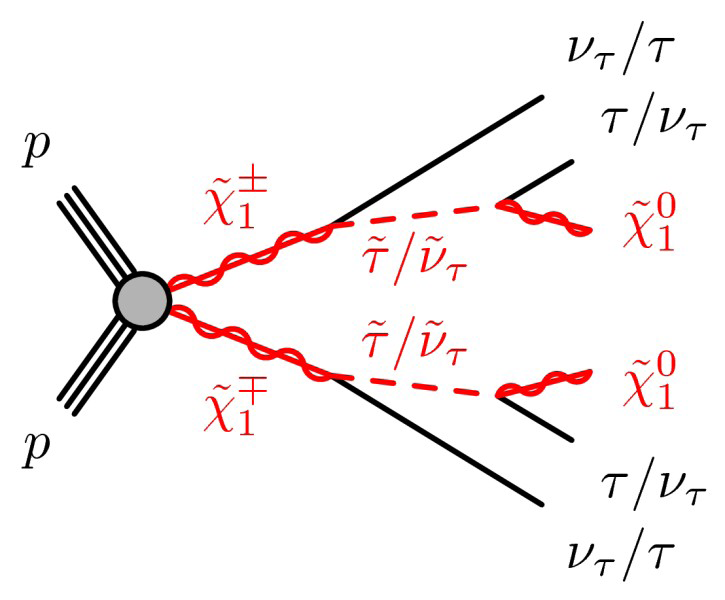
\includegraphics[width=0.3\textwidth]{Introductionfigs/DiChargino.png}
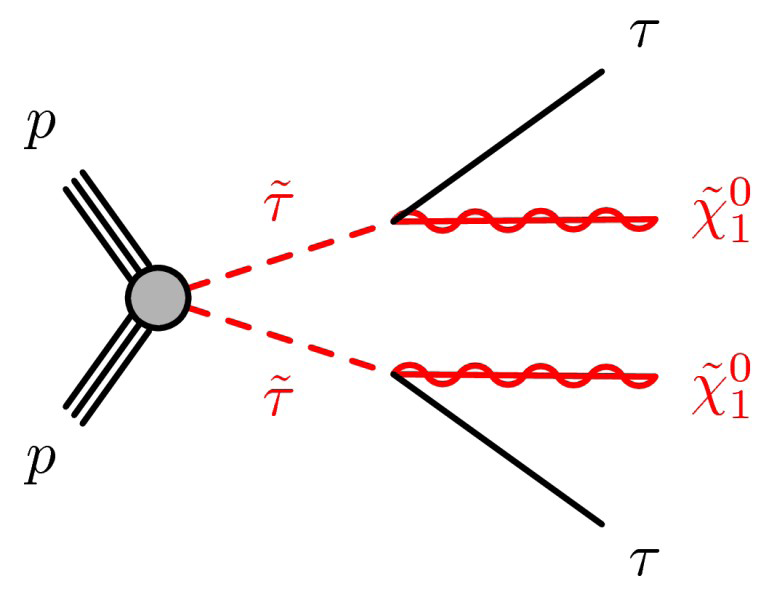
\includegraphics[width=0.3\textwidth]{Introductionfigs/DiSTau.png}
\caption{Schematic production of double tau from chargino pair and stau pair.}
\label{fig:Productions}
\end{figure}

The tau leptons can decay to electron or muon in 35\% of the cases (17.5\% for each lepton) 
or can decay via hadrons in 65\% of the cases. Since there are two leptons in the final state, then the probability of having 
two hadronic tau, \tauTau is 42\% and Lepton-\Tau is 46\%. We will see that having less background in \tauTau channel, makes it more powerful
in the final exclusion, although the branching ratio is a little lower.

The search variable which is used to distinguish between the signal and background is the stransverse mass (\mttwo) 
which is the natural extension of the known transverse mass (\mt) to a case 
when two massive particles with equal mass are created in pairs and decay via a chain of jets and leptons to two 
invisible particles. 
In the case of R-Parity conserving SUSY, the Lightest Supersymmetric Particle (LSP) escapes the detection and appears as 
a missing transverse momentum.
The distribution of \mttwo reflects the mass difference between the produced particles and the invisible  particles and is higher for sparticles
compared to the SM particles. Hence, SUSY should appear as an excess in the tail of the \mttwo distribution.
It was shown previously \cite{Chatrchyan:2012jx} that \mttwo is a powerful variable to search for SUSY. 




After introduction in the next section the \mttwo variable is introduced. 





\section{Experimental setup, event reconstruction and data sets}
\label{sect:CMSRec}


The central feature of the CMS apparatus is a superconducting solenoid of 6\unit{m} internal diameter, providing a magnetic field of 3.8\unit{T}. Within the superconducting solenoid volume are a silicon pixel and strip tracker, a lead tungstate crystal electromagnetic calorimeter (ECAL), and a brass and scintillator hadron calorimeter (HCAL), each composed of a barrel and two endcap sections. Muons are measured in gas-ionization detectors embedded in the steel flux-return yoke outside the solenoid. Extensive forward calorimetry complements the coverage provided by the barrel and endcap detectors. 
A more detailed description of the CMS detector, together with a definition of the coordinate system used and the relevant kinematic variables, can be found in reference \cite{Chatrchyan:2008zzk}.
%The object definition of this analysis is very close to the object reconstruction and identification in $H\to\tau\tau$ analysis previously published \cite{Khachatryan:2014wca}.
For completeness, a short review is given here. 


%An average of 21 $\Pp\Pp$ interactions occurred per LHC bunch crossing in 2012.
%For each reconstructed collision vertex the sum of the  $\pt^2$ of all tracks associated to the vertex is computed and the one with the largest value is taken as the primary collision vertex, where $\pt$ is the transverse momentum. The additional $\Pp\Pp$ collisions are referred to as pileup. 
Events from pp interactions must satisfy the requirements of a two-level trigger system.
The first level (L1) of the CMS trigger system, composed of custom hardware processors, uses information from the calorimeters and muon detectors to select the most interesting events in a fixed time interval of less than 4\mus. The high-level trigger (HLT) processor farm further decreases the event rate from around 100\unit{kHz} to around 400\unit{Hz}, before data storage. 

The particle-flow event algorithm~\cite{CMS-PAS-PFT-09-001,CMS-PAS-PFT-10-001} reconstructs and identifies each individual particle with an optimized combination of information from the various elements of the CMS detector. The energy of photons is directly obtained from the ECAL measurement, corrected for zero-suppression effects. The energy of electrons is determined from a combination of the electron momentum at the primary interaction vertex as determined by the tracker, the energy of the corresponding ECAL cluster, and the energy sum of all bremsstrahlung photons spatially compatible with originating from the electron track. The energy of muons is obtained from the curvature of the corresponding track. The energy of charged hadrons is determined from a combination of their momentum measured in the tracker and the matching ECAL and HCAL energy deposits, corrected for zero-suppression effects and for the response function of the calorimeters to hadronic showers. Finally, the energy of neutral hadrons is obtained from the corresponding corrected ECAL and HCAL energy. 

Jets are reconstructed with the anti-\kt clustering
algorithm~\cite{Cacciari:2008gp} with a distance parameter of 0.5. We apply
\pt- and $\eta$-dependent corrections to account for residual
effects of non-uniform detector response~\cite{Chatrchyan:2011ds}.
A correction to account for multiple pp collisions within the same or a nearby
bunch crossing (pileup interactions) is estimated on an event-by-event basis using the
jet-area method described in Ref.~\cite{cacciari-2008-659}, and is
subtracted from the reconstructed jet \pt.
The combined secondary vertex algorithm is used to identify (``btag'') jets 
originating from b-quarks.  This algorithm 
 is based on the reconstruction of secondary vertices, together with track-based lifetime information~\cite{Chatrchyan:2012jua}. 
In this analysis the "medium" working point is used. The working point corresponds to an average btagging efficiency of 70\%, 
light-quark jet misidentification rate of 1.5\%, and $\cPqc$-quark jet misidentification rate of 20\% 
for jets with a \pt\ value greater than 60\GeV.
Jets with  \PT $>$ 40 \GeV and $\abs{\eta} < 5.0$ and b-tagged jets with \PT $>$ 20 \GeV and $\abs{\eta} < 2.4$ are considered in this analysis.
% {\bf (Do you really use jets up to 5.0 in eta?)} 


The particles from the particle-flow algorithm are used to reconstruct the missing transverse energy vector $\VEtmiss$, defined as the negative of the vector sum of the transverse momenta of all reconstructed particles.  Corrections are applied to insure consistency between
$\VEtmiss$ and the corrections to jet energies described above.  The missing transverse energy in the event (\MET) is defined as the magnitude of $\VEtmiss$.

%The ECAL energy resolution for electrons with $\ET {\approx} 45$\GeV from $\Z \rightarrow \Pe \Pe$ decays is better than 2\% in the central region of the ECAL barrel $(\abs{\eta} < 0.8)$ where pseudorapidity $\eta$ is defined as $\eta = -ln [tan(\theta/2)]$,  $\theta$ being 
%the polar angle of the particle's track with respect to the counterclockwise beam direction. The resulotion is between 2\% and 5\% elsewhere. For low-bremsstrahlung electrons, where 94\% or more of their energy is contained within a $3 \times 3$ array of crystals, the energy resolution improves to 1.5\% for $\abs{\eta} < 0.8$~\cite{CMS:2013hoa}. 
%Muons are measured in the pseudorapidity range $\abs{\eta}< 2.4$, with detection planes made using three technologies: drift tubes, cathode strip chambers, and resistive plate chambers. Matching muons to tracks measured in the silicon tracker results in a relative transverse momentum resolution for muons with $20 <\pt < 100\GeV$ of 1.3--2.0\% in the barrel and better than 6\% in the endcaps, The \pt resolution in the barrel is better than 10\% for muons with \pt up to 1\TeV~\cite{Chatrchyan:2012xi}. 


%Jets are reconstructed offline from the energy deposits in the calorimeter towers, clustered by the anti-$k_\mathrm{t}$ algorithm \cite{Cacciari:2008gp, Cacciari:2011ma} with a size parameter of 0.5. In this process, the contribution from each calorimeter tower is assigned a momentum, the absolute value and the direction of which are given by the energy measured in the tower, and the coordinates of the tower. The raw jet energy is obtained from the sum of the tower energies, and the raw jet momentum by the vectorial sum of the tower momenta, which results in a nonzero jet mass. The raw jet energies are then corrected to establish a relative uniform response of the calorimeter in $\eta$ and a calibrated absolute response in transverse momentum \pt. 


Hadronically-decaying $\tau$ leptons (\Tau) are reconstructed using the hadron-plus-strips algorithm~\cite{Chatrchyan:2012zz}. The constituents of the reconstructed jets are used to identify individual tau decay modes with one charged hadron and up to two neutral pions, or three charged hadrons. The presence of extra particles within the jet, not compatible with the reconstructed decay mode of the $\Pgt$, is used as a criterion to discriminate \Tau from jets. Additional discriminators are used to separate \Tau from electrons and muons.
Prompt $\tau$ leptons are expected to be isolated in the detector.
%while leptons from heavy-flavor (c and b) decays and decays in flight are expected to be found inside jets. 
To discriminate them from QCD jets we use a measure of isolation 
based on the charged hadrons, photons, and neutral hadrons falling within 
a cone around the tau momentum direction.  A similar isolation algorithm is 
used in this analysis to separate leptons ($e$ or $\mu$) from tau decay from 
those arising in QCD processes.

%Electron, muon, and tau lepton isolation are estimated as
%\begin{equation}\begin{aligned}
%I_{\Pe,\Pgm} &=  \sum_{\rm charged}  \pt + \text{max}\left( 0, \sum_{\rm neutral}  \pt
%                                        +  \sum_{\gamma} {\pt} - 0.5 \sum_{\rm charged, pileup} \pt  \right ), \\
%I_{\Tau} &=  \sum_{\rm charged}  \pt + \text{max}\left( 0, \sum_{\gamma} {\pt} - 0.46 \sum_{\rm charged, pileup} \pt  \right ),
%\label{eq:reconstruction_isolation}
%\end{aligned}\end{equation}
%where $\sum_\text{charged}\pt$ is the scalar sum of the transverse momenta of the charged hadrons, electrons, and muons from the primary vertex located in a cone centered around the lepton direction of size $\Delta R = \sqrt{(\Delta\eta)^2+(\Delta\phi)^2}$ of 0.4 for electrons and muons and 0.5 for tau leptons.
%The sums $\sum_\text{neutral}\pt$ and $\sum_{\gamma} \pt$ represent the same quantities for neutral hadrons and photons, respectively. In the case of electrons and muons the innermost region is excluded
%to avoid the footprint in the calorimeter of the lepton itself from entering the sum. Charged particles close to the direction of the electrons are excluded as well, to prevent tracks originating from the conversion of photons emitted by the bremsstrahlung process from spoiling the isolation. In the case of \Tau, the particles used in the reconstruction of the lepton are excluded. The contribution of pileup photons and neutral hadrons
%is estimated from the scalar sum of the transverse momenta of charged hadrons from pileup vertices in the isolation cone $\sum_\text{charged, pileup}$. This sum is multiplied by a factor of 0.5 that approximately corresponds to the ratio of neutral-to-charged hadron production in the hadronization process of inelastic $\Pp\Pp$ collisions. In the case of \Tau, a value of 0.46 is used, as the neutral hadron contribution is not used in the computation of $I_{\Tau}$. An $\eta$, \pt, and lepton-flavor dependent threshold on the isolation variable is applied.

%In order to mitigate the effects of pileup on the reconstruction of \MET, a multivariate regression correction is used where the inputs are separated in those components coming from the primary vertex and those which are not~\cite{CMS-JME-12-002}.
%The correction improves the \MET resolution in $\cPZ\to\Pgm\Pgm$ events by roughly a factor of two in the case where 25 additional pileup events are present.

The $\cPZ$+jets, \wjets, $\cPqt\cPaqt$, and di-boson backgrounds to this search  are generated using the \MADGRAPH 5.1~\cite{Alwall:2011uj} generator.
Single-top-quark and Higgs background events are generated by {\POWHEG} 1.0~\cite{Nason:2004rx,Frixione:2007vw,Alioli:2009je,Alioli:2010xd}.
For parton shower and fragmentation, all generators are interfaced with \PYTHIA 6.4~\cite{Sjostrand:2006za}.
\PYTHIA is also used to generate signal events (chargino pair-production). To improve on the modeling of $\Pgt$ decays, we use the  \TAUOLA~\cite{Davidson:2010rw} package.
In the dataset considered in this paper,
there were on average 21 proton-proton interactions (``pileup'') in each bunch-crossing.
Consequently, additional interactions are generated with \PYTHIA and superimposed on Monte Carlo events in a manner consistent with the
luminosity profile of the dataset.
The detector response in the Monte Carlo background event samples is modelled by a
detailed simulation
of the CMS detector based on {\GEANTfour}~\cite{Agostinelli:2002hh}.  On the other hand, in order to reduce  computational requirements, signal events 
are processed by the CMS fast simulation \cite{Abdullin:2011zz} instead of {\GEANTfour}. 
All simulated events are reconstructed with the same algorithms as collision data.
The SM backgrounds are normalized using the most accurate calculations of the cross sections available,
generally with next-to-leading-order (NLO)
accuracy~\cite{Campbell:2012uf,Campbell:2011bn,xsec_WZ}.
The \textsc{Resummino}~\cite{Fuks:2012qx,Fuks:2013vua,Fuks:2013lya} calculations at NLO+NLL are used to calculate the signal cross sections, where 
NLL refers to next-to-leading-logarithmic precision.






\section{\texorpdfstring{The definition of $\rm {\mttwo}$}{The definition of MT2}}
\label{sect:mt2def}
The $\mttwo$ variable~\cite{Lester:1999tx,Barr:2003rg} is used in this analysis to discriminate between the SUSY signal and the SM backgrounds as proposed in~\cite{Barr:2009wu}. The variable was originally introduced to measure the mass of primary pair-produced particles, decaying eventually to undetected particles (e.g. neutralinos). Assuming the two primary supersymmetric particles undergo the same decay chain with visible and undetectable particles in the final state, the system can be described by the visible mass ($\mvisi$), transverse energy ($\etvisi$), and transverse momentum ($\vptvisi$) of each branch ($i=1,2$), together with the 
missing transverse momentum (\ptvecmiss) which is shared between the two decay chains. The \ptvecmiss is interpreted as the sum of the transverse momenta
of the neutralinos, $\vec{p}_{\rm T}^{\PSGczDo(i)}$.
However, in practice, in decay chains with neutrinos, \ptvecmiss includes contributions from the $\pt$'s of the neutrinos.
% $\pt^{\nu}$'s.

The transverse mass of each branch can be written as 
\begin{linenomath}
\begin{equation}
\label{eq:mtdef}
(\mt^{(i)})^{2}= (\mvisi)^2+m^2_{\PSGczDo}+2(\etvisi\et^{\PSGczDo(i)}-{\vptvisi}.\,{\vec{\pt}^{\PSGczDo(i)}}).
\end{equation}
\end{linenomath}

\noindent Using the correct neutralino mass, this distribution has an endpoint at the mass of the primary particle~\cite{Arnison:1983rp,Banner:1983jy,Affolder:2000bpa,Abazov:2002bu}. 
% similar to the W boson transverse mass used to measure $m_{\rm W}$
%As a generalization of the transverse mass, the $\mttwo$ variable is proposed to overcome the problem of unknown $\pt^{\PSGczDo(i)}$. The kinematic endpoint of $\mttwo$ carries model independent information about the mass difference between the primary and the secondary particles. 
For a given $m_{\PSGczDo}$, the $\mttwo$ variable is defined as
\begin{linenomath}
\begin{equation}
\label{eq:mt2def}
\mttwo(m_{\PSGczDo})= \min_{\vec{p}_{\rm T}^{\PSGczDo(1)}+\vec{p}_{\rm T}^{\PSGczDo(2)}=\ptvecmiss}\,\left[\,\max\,\{ \, \mt^{(1)},\,\mt^{(2)}\,\}\,\right].
\end{equation}
\end{linenomath}

For the correct value of $m_{\PSGczDo}$, the kinematic endpoint of the $\mttwo$ distribution is at the mass of the primary particle, and it shifts accordingly when the assumed $m_{\PSGczDo}$ is lower or higher than the correct value. In this analysis we set
$m_{\PSGczDo}=\mvisi=0$.
The visible part of the decay chain consists of either the two hadronically decaying tau leptons ($\hadtau \hadtau$ channel)
or a combination of a muon or an electron with a $\hadtau$ candidate ($\leptonTau$ channel).

%With our choices of $m_{\PSGczDo}$ and $\mvisi$, the resulting $\mttwo$ 
%in back-to-back events (e.g., QCD di-jets) is close to zero, regardless of the values of $\MPT$ and the $\pt$ of the $\tau$ candidates.
%This is to be contrasted with the case of signal where the taus or leptons are in general not back-to-back 
%due to the presence of two undetected neutralinos.
%the visible system is not back-to-back and  \mttwo has larger values.
%variable is expected to well reject not only events with no genuine $\MPT$ but events with a back-to-back topology ($\mttwo=0$) . 

With  our choices of $m_{\PSGczDo}$ and $\mvisi$, the resulting \mttwo value is close to zero for back-to-back topology of \tauTau or \leptonTau  
events (e.g., Drell-Yan events; QCD di-jets if two jets are misidentified as \Tau objects), regardless of the values of \MPT and the \PT of 
the tau candidates. This is not the case for signal events where the taus or leptons are generally not in back-to-back topology due 
to the presence of two undetected neutralinos.

The distribution of \mttwo reflects the scale of the produced particles and is much higher for heavy sparticles
compared to the lighter SM particles. Hence, SUSY 
could manifest itself
as an excess of events in the high-side tail of the \mttwo distribution.
% It was shown previously \cite{Khachatryan:2014qwa} and \cite{Chatrchyan:2012jx}    
% that \mttwo is a powerful variable to search for SUSY in both leptonic and hadronic final states.

\section{\texorpdfstring{Event selection for the \tauTau channel}{Event selection for the tau-tau channel}}
\label{sect:tauTauCuts}
In this channel data of proton-proton collisions,  corresponding to an integrated luminosity of 18.1 $\mathrm{fb}^{-1}$, are used.
The events are first selected with a trigger \cite{Chatrchyan:2011nv} that requires the presence of
two \Tau candidates with \PT $>$ 35\GeV and $|\eta|<$ 2.1, which pass loose identification and isolation criteria.

Offline, %the measure of isolation of the two \Tau candidates must be less than 1.5\GeV (medium working point
%of the $\tau$ isolation discriminator \cite{Khachatryan:2015dfa}), 
the two \Tau candidates must pass the tight $\tau$ isolation discriminator,
\PT $>$ 45\GeV and $|\eta|<$ 2.1, and have opposite electric charge (OS).
In events with more than one \tauTau pair, we only consider the pair with the most isolated \Tau objects. 

Events with extra isolated electrons or muons of \PT $>$ 10\GeV and $|\eta| <$ 2.4 
are rejected to suppress %the contribution of the associatiated production of \Z with vector bosons.
backgrounds from diboson decays.
Inspired from the MC studies, to reduce the contribution of the \Z$ \rightarrow$ \tauTau backgrounds, events are  rejected where the visible
di-\Tau invariant mass is between 55 and 85\GeV (\Z boson veto).  
Furthermore, contributions from low-mass DY and QCD multijet production are 
reduced by requiring the invariant mass to be greater than 15\GeV.
Moreover, to further reduce \Z $\rightarrow$ \tauTau and QCD multijet events, %the loose requirements 
\MPT $>$ 30\GeV and \mttwo $>$ 40\GeV are also required.
The minimum angle \deltaphi in the transverse plane between the \ptvecmiss and any of the \Tau and jets, 
including b-tagged jets, must be greater than 1.0 radians. 
This requirement reduces backgrounds from QCD multijet events and \wjets events.

After applying the preselection described above,
additional requirements are introduced to define two search regions.
The first search region (\binone) targets models with large mass difference ($\Delta m$) 
between charginos and neutralinos.
In this case, the \mttwo signal distribution can have a long tail beyond the 
distribution of SM backgrounds.
The second search region (\bintwo) is dedicated to models with small values of $\Delta m$.
In this case, the sum of the two transverse mass values, \SumMT = $\mt(\Tau^1,\ptvecmiss) + \mt(\Tau^2,\ptvecmiss)$, 
provides additional discrimination between signal and SM background processes.

The two signal regions (SR) are defined as:
\begin{itemize}
\item {\bf \binone}: \mttwo $>$ 90\GeV,
\item {\bf \bintwo}:  \mttwo $<$ 90\GeV, \SumMT $>$ 250\GeV, and b-tagged jets are vetoed.
\end{itemize}
The veto on b-tagged jets in SR2 reduces the
\ttbar events, which
are expected in  the low-\mttwo region. Table \ref{Tab.Cuts} summarizes the selection requirements for different signal regions.
\begin{table}[!htb]
\begin{center}
\caption{Definition of signal regions.}
\begin{tabular}{|c|c|c|}
\hline
               & \tauTau & \tauTau               \\
   \leptonTau  & \binone & \bintwo               \\\hline\hline
 OS \leptonTau & \multicolumn{2}{c|}{OS \tauTau}  \\\hline
\multicolumn{3}{|c|}{Extra lepton veto}          \\\hline
\multicolumn{3}{|c|}{Invariant mass of \leptonTau or \tauTau $>$ 15\GeV}\\\hline
\multicolumn{3}{|c|}{\Z boson mass veto}              \\\hline
\multicolumn{3}{|c|}{\MPT $>$ 30\GeV}            \\\hline
\multicolumn{3}{|c|}{\deltaphi $> 1.0 $ radians}         \\\hline
\multicolumn{3}{|c|}{$\mttwo > 40\GeV$}         \\\hline
b-tagged jet veto&  - & b-tagged jet veto  \\\hline
\multicolumn{2}{|c|}{$\mttwo > 90\GeV$} & $\mttwo < 90\GeV$ \\\hline
$\tauMT > 200\GeV$    &  - & $\SumMT > 250\GeV$ \\\hline
\end{tabular}
\label{Tab.Cuts}
\end{center}
\end{table}
%The distributions of $\mttwo$ and $\SumMT$ for data and the SM prediction are shown in Fig.~\ref{fig:comparison} before the application of the final requirements listed above. In the $\SumMT$ distribution, the b-tagged jets are vetoed and \mttwo $<$ 90\GeV is also applied. The SM predictions in Fig.~\ref{fig:comparison} are from simulated events, except for the QCD multijet prediction which is taken from same-sign di-tau data events, after subtracting a small contribution of same-sign non-QCD events estimated from Monte Carlo events. The data and SM predictions are in agreement within the statistical uncertainties.
%The expected distributions for a SUSY signal corresponding to a moderate mass difference $(m_{\chione}=240\GeV,~m_{\PSGczDo}=40\GeV)$ are also shown for illustration purposes.
%\begin{figure}[!htb]
%\centering
%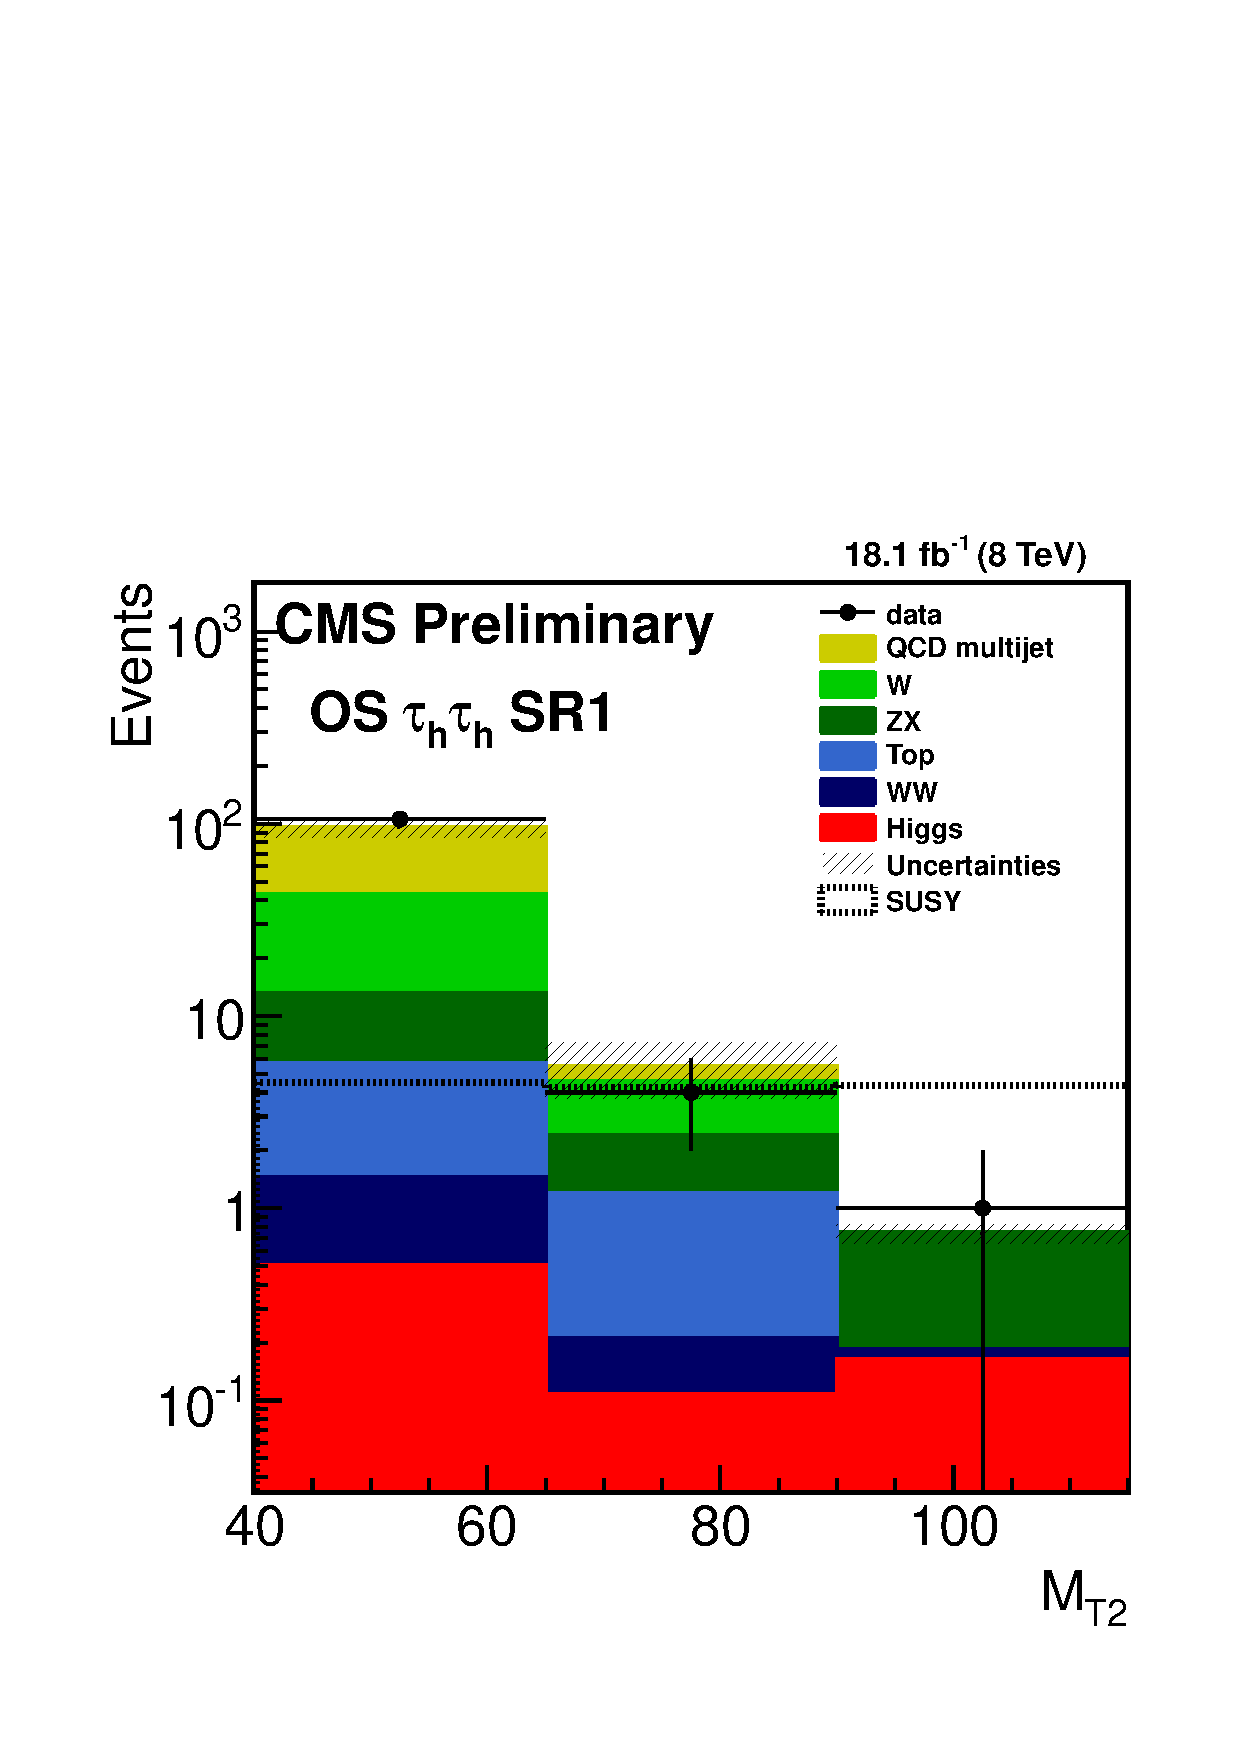
\includegraphics[angle=0,scale=0.375]{TauTauFigs/MT2.pdf}
%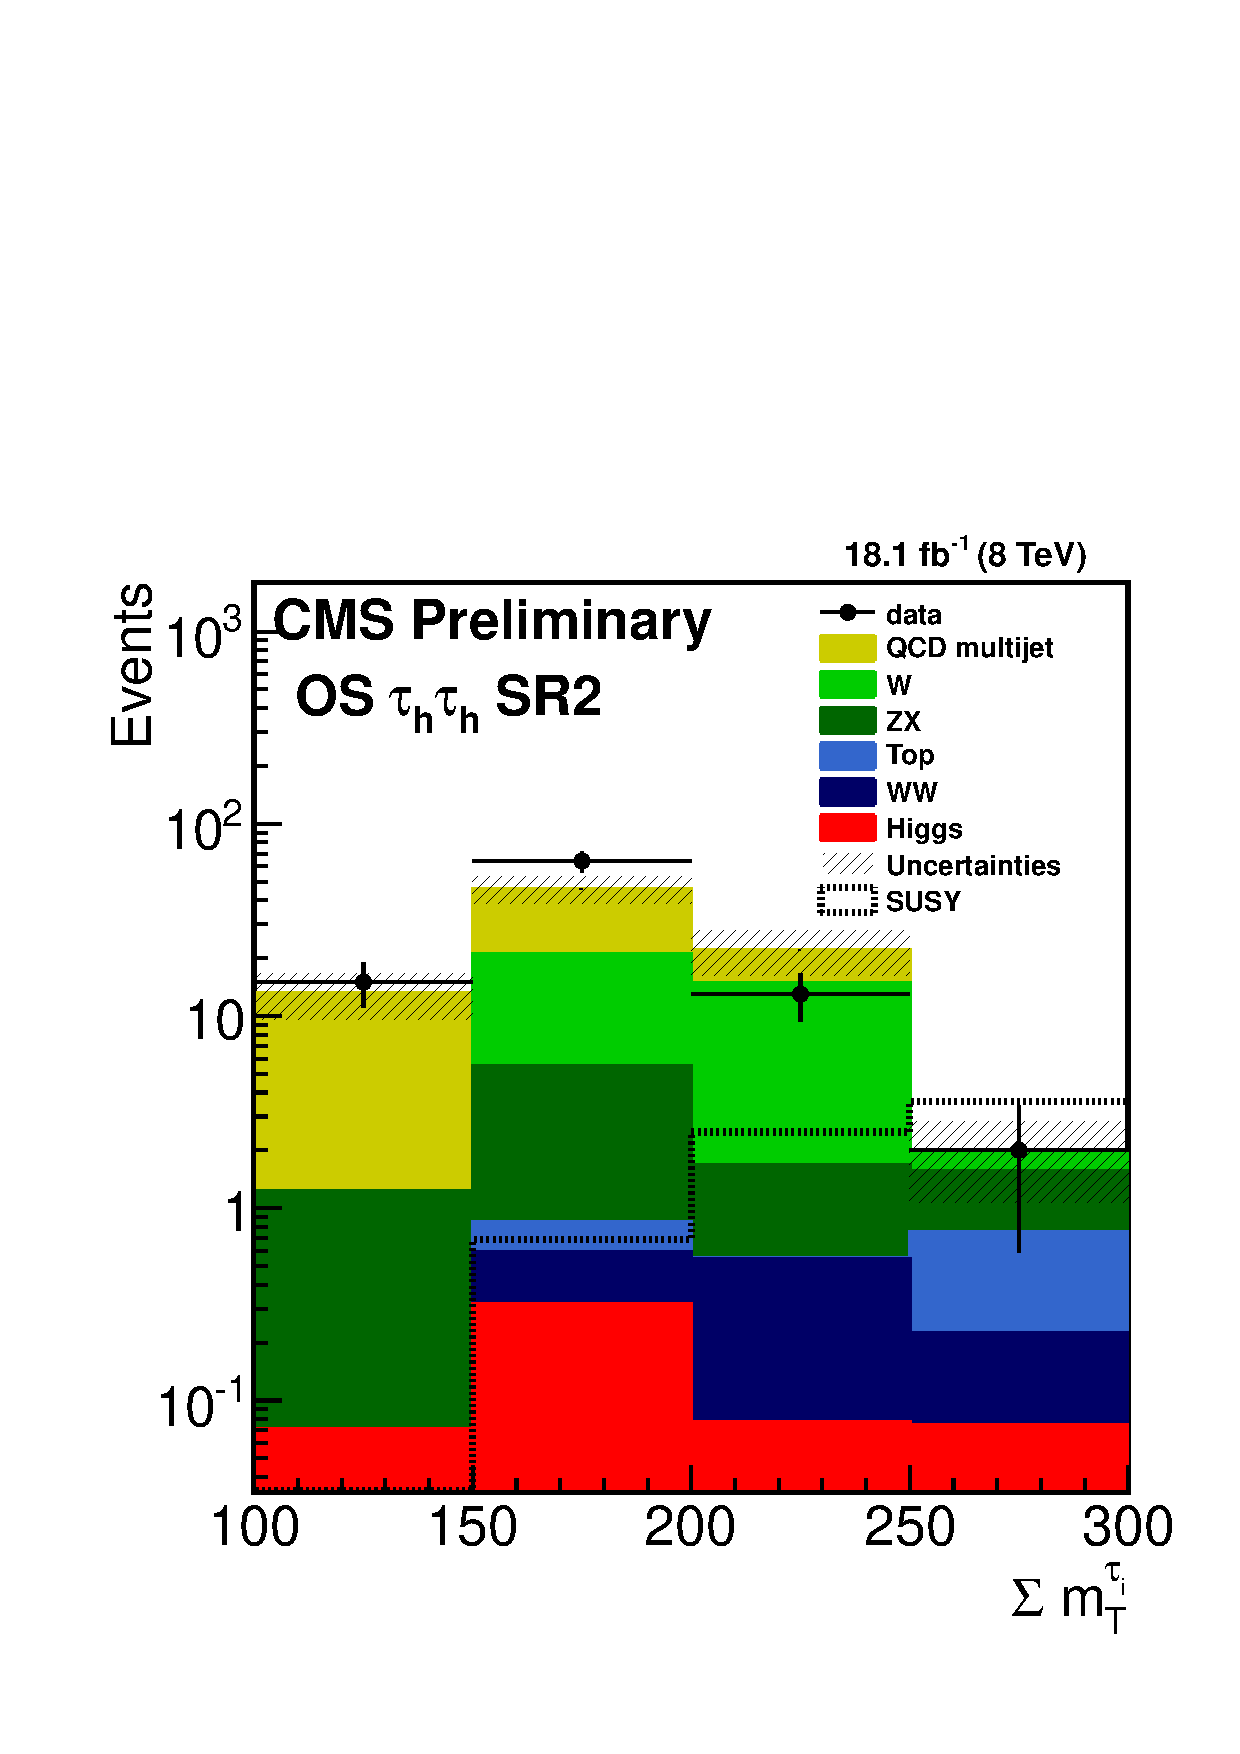
\includegraphics[angle=0,scale=0.375]{TauTauFigs/SumMT.pdf} \\ 
%\caption{The distributions of \mttwo (left) and \SumMT (right) after applying all the selections. 
%The last bins of the histograms correspond to the two signal regions (\binone and \bintwo). The signal distribution is shown for $m_{\chione}=240\GeV,~m_{\PSGczDo}=40\GeV$.}
%\label{fig:comparison}
%\end{figure}

\section{\texorpdfstring{Event selection for the \leptonTau channel}{Event selection for the lepton-tau channel}}
\label{sect:eleTauCuts}
Events for the \leptonTau final states (e\Tau and $\mu\Tau$)
were collected with triggers that require 
a loosely isolated \Tau with \PT $>$ 20\GeV and $|\eta|$ $<$ 2.3 as well as
an isolated electron or muon with $|\eta| < 2.1$.  The minimum
\PT requirement for the electron (muon) was increased during the data taking from 20 to 22\GeV (17 to 18\GeV)
due to the increase in instantaneous luminosity.

In the offline analysis, the electron, muon, and \Tau objects are required to have \PT $>$ 25, 20, and 25\GeV, respectively, 
while tightening the corresponding identification and isolation requirements.
In events with more than one opposite-sign \leptonTau pair, we only consider
 the pair that maximizes the scalar sum of \Tau and electron or muon 
transverse momenta.  Events with an additional loosely isolated lepton
with \PT $>$ 10\GeV are rejected to suppress backgrounds from $Z$ boson
decays.  

Just like for the \Tau\Tau channel, we apply preselection requirements to suppress
QCD multijet, \ttbar, $Z \to \tau \tau$ decays, and low mass resonance events.
These requirements are: \mttwo $>$ 40\GeV, \MPT $>$ 30 GeV, \leptonTau 
invariant mass between 15 and 45\GeV or $>$ 75\GeV, \deltaphi $>$ 1, and we veto events with b-tagged jets.
The final signal region requirements are \mttwo $>$ 90\GeV and 
\tauMT $>$ 200\GeV. %where \tauMT is the \Tau transverse mass 
The latter requirement provides discrimination against the \wjets background.  Unlike the \tauTau channel,
events with \mttwo $<$ 90\GeV are not used because of the higher 
level of background. Table \ref{Tab.Cuts}
\begin{table}[!htb]
\begin{center}
\caption{Definition of different signal regions. OS stands for opposite-sign pairs.}
\begin{tabular}{|c|c|c|}
\hline\hline
               & \tauTau & \tauTau               \\
   \leptonTau  & \binone & \bintwo               \\\hline\hline
 OS \leptonTau & \multicolumn{2}{c|}{2 OS \Tau}  \\\hline
\multicolumn{3}{|c|}{\MPT $>$ 30\GeV}            \\\hline
\multicolumn{3}{|c|}{Extra Lepton Veto}          \\\hline
\multicolumn{3}{|c|}{Invariant mass of \leptonTau or \tauTau $>$ 15\GeV}\\\hline
\multicolumn{3}{|c|}{\Z boson veto}              \\\hline
\multicolumn{3}{|c|}{\deltaphi $> 1$}         \\\hline
\multicolumn{3}{|c|}{$\mttwo > 40 \GeV$}         \\\hline
\multicolumn{2}{|c|}{b-tagged jets vetoed}&  -   \\\hline
\multicolumn{2}{|c|}{$\mttwo > 90 \GeV$} & $\mttwo < 90 \GeV$ \\\hline
$\tauMT > 200 \GeV$    &  - & $\SumMT > 250\GeV$ \\\hline\hline
\end{tabular}
\label{Tab.Cuts}
\end{center}
\end{table}
summarizes the selection requirements for different signal regions.


Figure \ref{fig:mt2leptontau} % and \ref{fig:taumtleptontau} 
shows the \mttwo distribution after the preselection.
%and the \tauMT distribution after the preselection and the \mttwo requirements, respectively.
The data are in good agreement with the SM expectations. A SUSY signal corresponding to a high mass difference 
 $(m_{\chione}=380\GeV,~m_{\PSGczDo}=1\GeV)$ is used to show the expected signal distribution.

\begin{figure}[!htb]
\centering
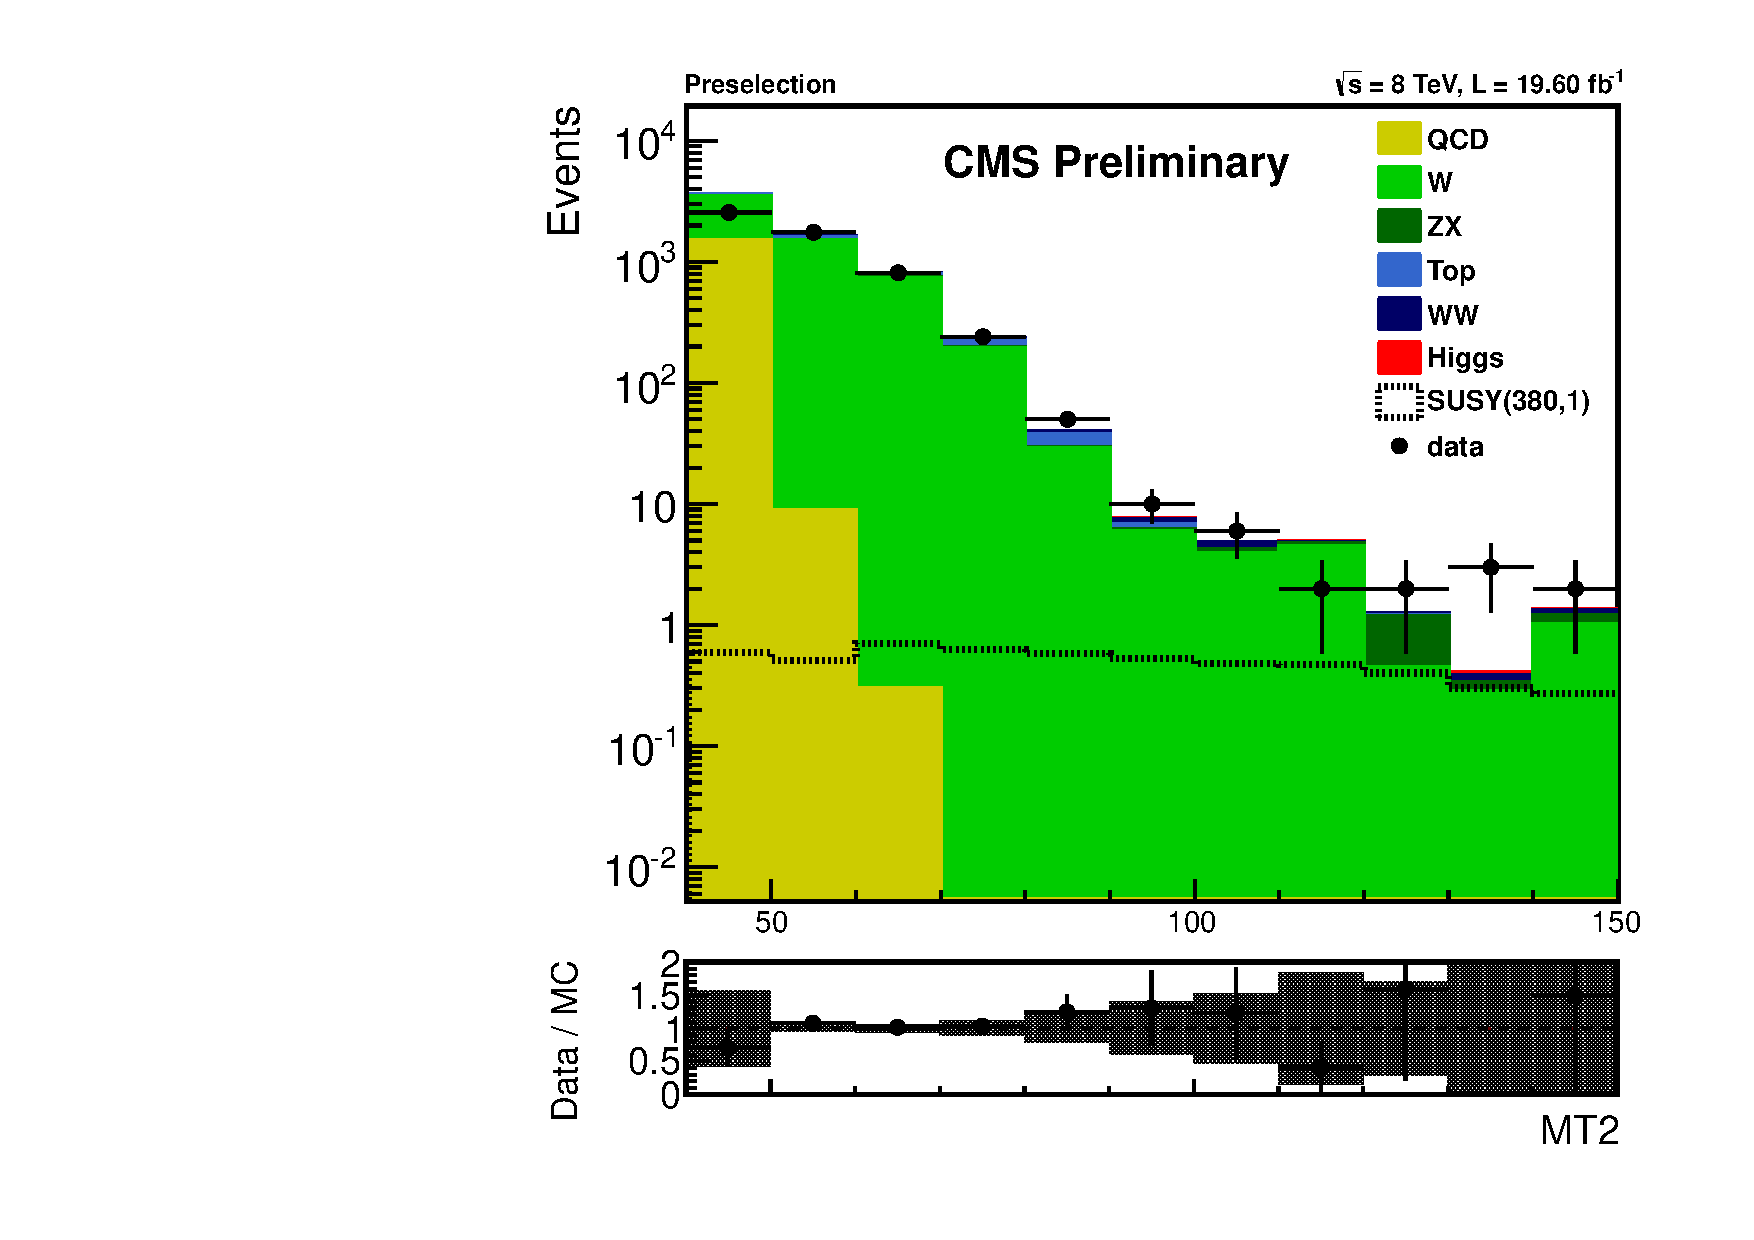
\includegraphics[angle=0,scale=0.375]{SelectionEleTau/MT2.pdf}
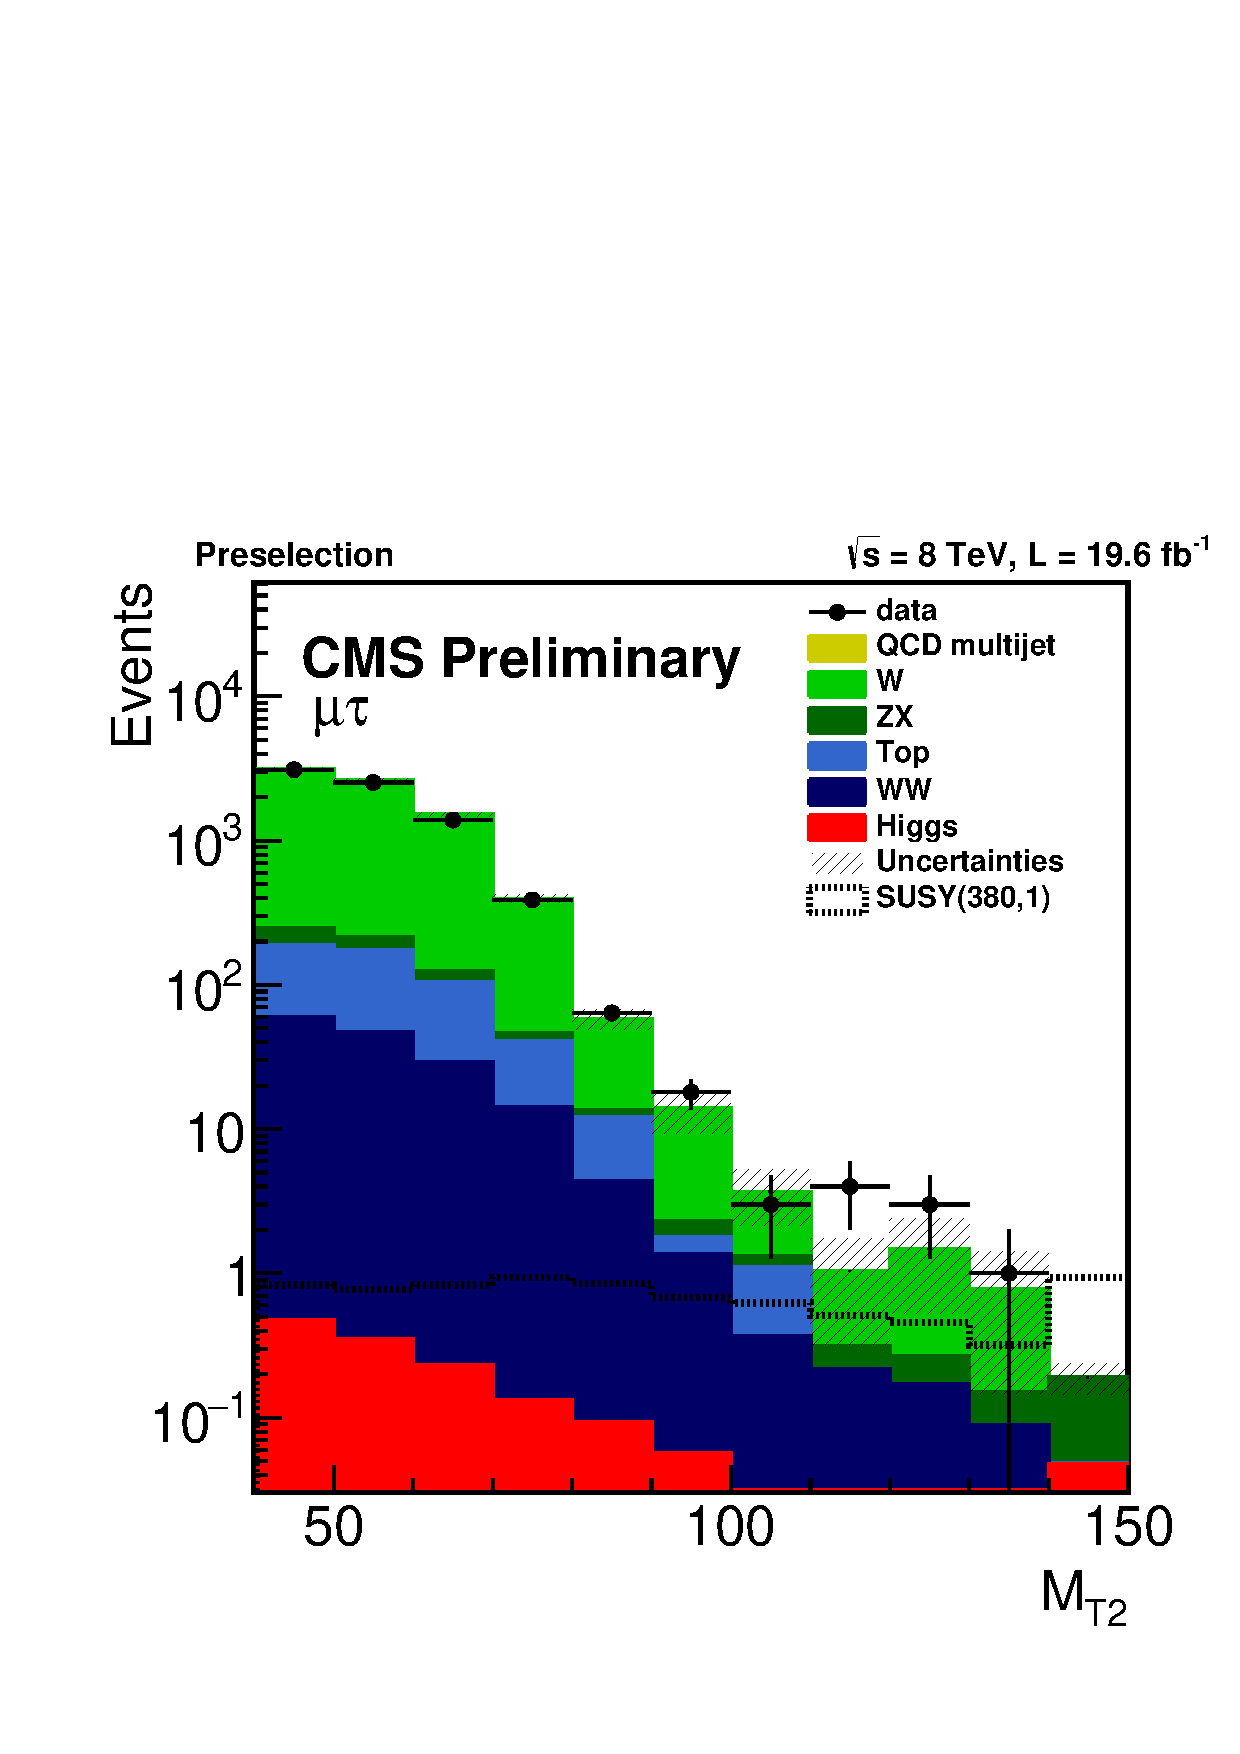
\includegraphics[angle=0,scale=0.375]{SelectionMuTau/MT2_Ratio_Preselection_unBlinded.pdf}
\caption{\mttwo  distributions for events in the preselection sample, compared to Monte Carlo events in (left) \eTau and (right) \muTau channels. The signal point shown here is $(m_{\chione}=380\GeV,~m_{\PSGczDo}=1\GeV)$.}
\label{fig:mt2leptontau}
\end{figure}


\section{Backgrounds}
\label{sect:bkgLepTau}
We separate the backgrounds into two distinct categories.  Those with 
``fake'' \Tau, i.e., events where a quark or gluon jet has been misidentified
as a \Tau, and those without \Tau misidentifications.  
The fake \Tau backgrounds arise mostly from QCD and $W+$ jets events.  The 
other backgrounds are from \ttbar, $Z+$ jets, dibosons, and Higgs decays.
Backgrounds with fake \Tau are estimated with data-driven methods; the 
remaining backgrounds are taken from Monte Carlo.

%In different channels, the contribution of the events with a fake \Tau, namely QCD and $W$jets is estimated using the data. 
%For the prompt \Tau's, from top, $\cPZ$jets, di-boson and higgs we trust 
%the MC, but the important contributions are validated in a signal like region. 
%In this section we will discuss the different background estimation techniques used.
%In continue, estimation of different backgrounds are explained.

\subsection{\texorpdfstring{QCD background estimation in the $\tauTau$ channel}{QCD background estimation in the tau-tau channel}}
%{\bf (I actually could not fully understand from the original text how this is done.
%I rewrote it extensively, according to my understanding, and I took out
%many details that I do  not think are relevant.  In particular, I 
%did not really understand the same-sign business.
%So I what I say about same-sign may be quite wrong).}

Events from QCD can enter the signal regions if two quark or gluon jets are 
misidentified as \Tau, and the rest of the kinematical cuts are also 
satisfied.  Isolation is an important 
discriminant between fake \Tau and prompt \Tau.
Therefore we define control regions in the 
\Tau pair isolation vs. \mttwo or \SumMT 
planes, as shown in Fig.~\ref{fig:ABCDQCD}. We then estimate the QCD background
in the signal regions starting from the event counts in the
control regions under the assumption
that for fake \tauTau the isolation is uncorrelated with \mttwo or \SumMT.
This assumption was checked in the QCD domainated region of data.
%{\bf (Not clear to me what isolation means here, because
%you have two \Tau and therefore two isolations.  Which of the 
%two isolations do you actually use?  This needs to be specified).}

To reduce contamination from prompt \tauTau, in the control regions with at least one loose \Tau, 
the same-sign pairs are selected.  Residual contributions from prompt
\tauTau and $W+$ jets are subtracted off based on Monte Carlo expectations.
In addition, the cut on $\Delta \Phi$
is removed to improve on the statistical power of the method. 
The final estimate of the background
is taken from the control regions extrapolation with corrections
associated with the same-sign requirement and the efficiency of 
the $\Delta \Phi$ requirement for QCD events.


%Due to the large cross section of the QCD multijet events and lack of the statistics, there is a large statistical uncertainty on the 
%yield of the QCD events from MC. On the other hand, 
%The QCD multijet events contribute to the signal selection of the \tauTau channel, when two jets are 
%fakely identified as \Tau's. The fake rate can be different between data and MC, so a data driven method is developed to estimate the 
%contribution of the QCD multijet events. 
%Since the search variable (\mttwo in \binone and \SumMT in \bintwo) and the 
%isolation of the \Tau's are uncorrelated in the QCD events, the ratio of the events selected by the signal cuts over the events 
%with loosely isolated \Tau's should be independent from the search variable, so one can find the ratio in the low \mttwo or \SumMT and 
%multiply it to the number of events in the control region which is defined same as the signal region except the \Tau's are loosely isolated. 
%This would give an estimate of the QCD events in the signal region. In the signal region, loosely isolated  \Tau's 
%($I_{\Tau} <$ 2 \GeV ) 
%are excluded, but in the control region, only the pairs with at least one loosely isolated \Tau are selected. 
%These pairs are requested to be same-sign to suppress the signal contamination. To further increase the statistics 
%in different regions, the cut on the minimum angle in the transverse plane between the \MET and the jets is removed. The final estimation
%is corrected by the efficiency of this cut which is read from data and will be described in continue.

%{\bf It seems to me that this procedure would at the same time estimate 
%the $W+$ jets background with one real \Tau and one fake \Tau. (??)}


\begin{figure}[!Hhtb]
\centering
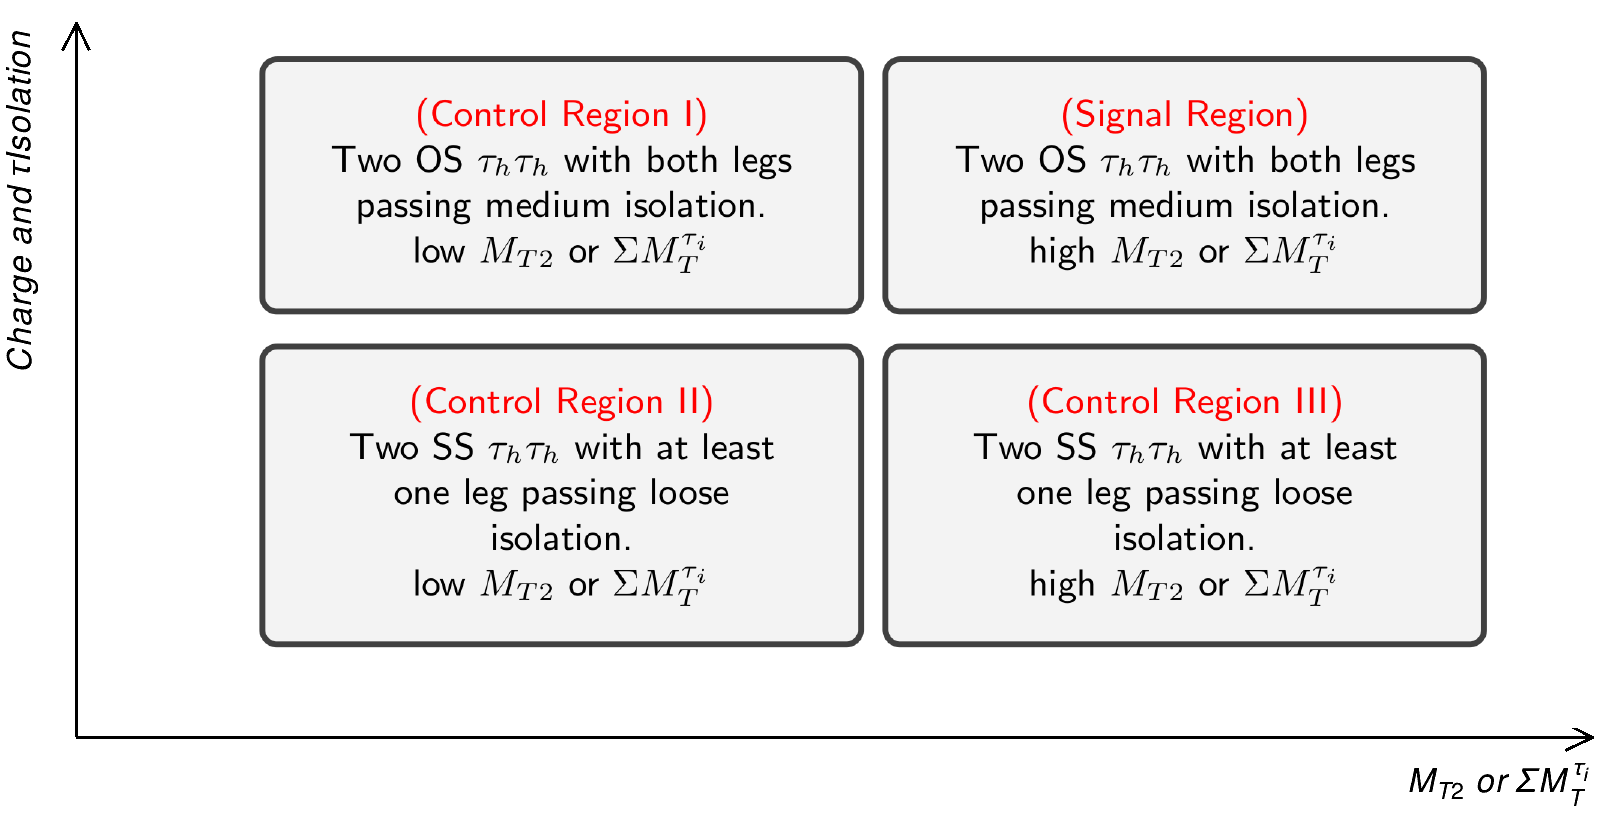
\includegraphics[angle=0,scale=0.30]{Bkg/ABCD.png}
\caption{Schematic description of the regions used to estimate the QCD backgrounds.}
\label{fig:ABCDQCD}
\end{figure}

%Non-QCD events from MC are subtracted from data to find a QCD sample.
%In the low \mttwo or \SumMT of the QCD sample, the ratio of the signal like events over the same-sign loose pairs 
%is found and verified to be flat as a function of the search variable. 
%A horizontal line is fitted to
%This ratio is multiplied to the same-sign loose pairs in high \mttwo or \SumMT and corrected by the efficiency of the 
%cut on the minimum angle between the \MET and the jets, to find the QCD contamination in the signal region. 
%The efficiency of the cut on the minimum angle between the \MET and the jets, is found with the same events as a function of the search variables.
%The value of the efficiency in the last bin in vicinity of the signal region is used to correct the estimation.
%To estimate the systematic uncertainty of the estimated value and take into account the potential correlation between the two values, 
%the method to extract the
%ratio and the efficiency are varied from approximating by a flat line to fitting by a straight line with a floating slope 
%or using the value of the  last bin before the signal region. 
%This is  also a measure  of the correlation between the two variables which are assumed to be uncorrelated. 


\begin{table}[!Hhtb]
\begin{center}
\begin{tabular}{|l|c|}
\hline\hline
 Region      &  Estimation\\
\hline\hline
%SR1      & 0.15 $\pm$ 0.22 $\pm$ 0.13 \\   
SR1      & 0.13 $\pm$ 0.19 $\pm$ 0.10 \\
\hline
%SR2      & 0.82 $\pm$ 0.65 $\pm$ 0.07  \\
SR2      & 1.15 $\pm$ 0.81 $\pm$ 0.25  \\
\hline\hline
\end{tabular}
\caption{The estmated QCD background in the \tauTau channel. The first uncertainty is statistical and systematic of the method, the second is systematic due to correlation assumptions.}
\label{4QCDbg}
\end{center}
\end{table}

Table \ref{4QCDbg} 
summarizes the estimation of the QCD background contribution in the two signal regions after extrapolation from the control regions and 
correcting for the $\Delta \Phi$ efficiency.  
The systematic uncertainties are associated with the uncertainty on the validity 
of the assumption that isolation and \mttwo or \SumMT are not correlated.
%${\bf (I think that this is what you had in the original text,
%but what about the efficiency of the $\Delta \Phi$ requirement and the 
%same-sign vs. opposite-sign business?)}


\subsection{\texorpdfstring{$W$jets background estimation in the $\tauTau$ channel}{Wjets background estimation in the tau-tau channel}}
%{\bf I did not understand this, so I did not try to edit it.  This background has one real \Tau and one fake \Tau.  So according to the claim that fake \Tau cannot be taken from MC, this should be data-driven.  But when I read this it seems like it is done from MC, with complications associated with the fact that you do not have enough statistics in the Monte Carlo.  So, I am confused.}
The contribution of the $W$jets background is taken from simulation. %with a large uncertainty. 
While in \bintwo region the number of simulated $W$jets events is large enough to provide a reliable estimate, in \binone no such events remain after the final requirement of \mttwo $>$ 90 \GeV. Therefore, a valid estimation for the efficiency of this requirement, $\epsilon_{\rm M_{T2}>90}$, is necessary to determine the $W$jets contamination in \binone region.

Since the size of the simulated $W$jets sample is not large enough to adequately populate our desired phase space, $\epsilon_{\rm M_{T2}>90}$ is calculated in a phase space with looser selection criteria. It is first evaluated in a $W$jets sample with a pair of oppsite-charge \Tau's where the \Tau candidates are selected similar to signal region. Additional signal selection requirements, such as lepton veto or $\mindphifour>1$, are applied one by one and $\epsilon_{\rm M_{T2}>90}$ is calculated at every step. The values are found to be close to each other; their wighted average is taken as the final estimate for $\epsilon_{\rm M_{T2}>90}$ with the weights corresponding to the size of the simulated sample at each step. The uncertainty on the \Tau energy scale introduces the largest variation on $\epsilon_{\rm M_{T2}>90}$. This variation is considered as a systematic uncertainty on the estimated efficiency.

The simulation of the $W$jets process is validated in a data control sample constructed based on the \muTau signal selection requirements. The selected \muTau pair in this region is required to be same-sign with a less strict \Tau isolation condition. Moreover, jets fulfilling the loose b jet identification criteria are vetoed and the \mttwo requirement is changed to $40<\mttwo<60\,\GeV$. The $W$jets events constitute more than 90\% of this control sample and the overall normalization from simulation is consistent with data, within uncertainties.

This control region is additionally used to check the data-simulation compatibility for the $\epsilon_{\rm M_{T2}>90}$ estimate. The \mttwo condition is modified to $\mttwo>40\,\GeV$ to allow for such investigation. The contribution of $W$jets events remains almost unchanged. The $\epsilon_{\rm M_{T2}>90}$ quantity is evaluated in data and simulation and the data-to-simulation ratio is used to correct the $\epsilon_{\rm M_{T2}>90}$ estimation in signal region. The difference between the predicted and measured $\epsilon_{\rm M_{T2}>90}$ is taken into account as an additional uncertainty. 

The final value for the contribution of $W$jets in this signal region is $0.69\pm0.54$.

%In \binone of the \tauTau channel, the number of remaining events for $W$jets from MC is zero, but it has a large statistical uncertainty due to lack of the statistics in the simulated sample. To have a better estimation of the Wjets contribution in the final yields, the yield before the last cut (\mttwo $>$ 90 \GeV) is multiplied by the efficiency of the cut. To find the efficiency, several cuts like lepton veto, \Z veto and the minimum angle in the transverse plane between the \MET and the jets are relaxed to have a high statistics sample. The cut efficiency is found in the exclusive samples that either fail or pass each relaxed cut to remove any correlation between the cuts and the \mttwo cut. 
%A horizontal line is fitted to the measured values to extract the cut efficiency. 
%The efficiencies are close to each other and the weighted average of the values is used as the final efficiency.
%The main source of the systematic uncertainty on the backgrounds 
%is the \Tau energy scale. The energy of the \Tau's is scaled up and down by one standard deviation and all related variables are 
%recalculated and the cut efficiency is measured on the new samples. 
%This variation due to the uncertainty of the \Tau energy scale is considered as the systematic uncertainty of the measured efficiency.
%To validate the MC prediction for Wjets against the data, a Wjets enriched sample is made in \muTau channel, 
%by rejecting the loosely tagged b-jets, relaxing the \Tau isolation from tight to loose and forcing the muon and \Tau to have the same-sign. 
%In the control sample, Wjets consist more than 90\% of the MC events. The normalization of the MC distribution  is found consistent with the data within the uncertainties, but the low statistics of MC does not allow to verify the efficiency of \mttwo $>$ 90 \GeV cut, so we correct the MC by the efficiency of data and the uncertainty of the correction is also conidered which is about 77\%. The final value for the contribution of $W$jets in this signal region is 0.69 $\pm$ 0.54.
%\subsection{\texorpdfstring{DY background estimation in the $\tauTau$ channel}{DY background estimation in the tau-tau channel}}
\subsection{\texorpdfstring{DY background estimation}{DY background estimation}}
This background is taken from Monte Carlo simulation.  The simulation is 
validated in a $\mu \tau$ control region obtained by removing the $\Delta \Phi$
requirement and by
inverting the Z-veto
(\mttwo $<$ 20 \GeV, 40 $<$ \tauMT $<$ 100 \GeV).  Note that the transverse momentum 
of the \Z system, which is correlated with 
\mttwo, is also well reproduced in simulation. Table \ref{Tab.DYbkg}
\begin{table}[!Hhtb]
\begin{center}
\begin{tabular}{|l|c|}
\hline\hline
Channel            &  DY Estimation\\
\hline\hline
\eTau              & 0.19  $\pm$  0.03  $\pm$ 0.05 \\\hline
\muTau             & 0.25  $\pm$  0.06  $\pm$ 0.06 \\\hline
\tauTau (SR1)      & 0.56  $\pm$  0.07  $\pm$ 0.14 \\\hline
\tauTau (SR2)      & 0.81  $\pm$  0.56  $\pm$ 0.20 \\
\hline\hline
\end{tabular}
\caption{DY background in different channels. The first uncertainty is statistical and the second is systematic.}
\label{Tab.DYbkg}
\end{center}
\end{table}
summarizes the DY contribution in different signal regions. 25\% systematic uncertainty is assigned to the central value 
which is discussed later. For $\ell\Tau$ channels, only the promot contributions are reported. 
A separate method is developed to estimate the fake contamination in these channels.
%{\bf At this point you need to give the results of this procedure, ie, the
%background predictions in the two regions, including systematics,
%just like you did in the previous sections.}

%The events containing a \Z boson can be an important background in different channels. To
%estimate this background, we use the simulated events. The simulation
%is validated in a Z-dominated control region.
%This region is defined in the \muTau channel by relaxing  the \Z veto cut, \mttwo $<$ 20 \GeV, 40 $<$ \tauMT $<$ 100 \GeV and 
%removing the cut on the minimum angle in the transverse plane between the \MET and the jets. Comparing the events under the \Z peak in data and MC 
%confirms that the normalization of the  MC is correct. To validate the shape in the signal region, 
%the transverse momentum of the \Z system is compared in data 
%and MC  and a good agreement is seen within the uncertainties. Due to the correlation between the \mttwo and \pt of the \Z system, we can trust the shape of the DY events from MC. 


\subsection{\texorpdfstring{Fake \Tau in the $\ell\Tau$ channels}{Fake tau the in lepton-tau channels}}

This contribution is estimated using a fake rate method.
When the loose signal selection is applied, the number of loose $\hadtau$'s ($L$) is:
\begin{equation}
L = P + F
\end{equation}
where $P$ is the number of prompt $\hadtau$'s and $F$ is the number of fake 
$\hadtau$'s. If the selection is tightened, the number of tight $\hadtau$'s (T) is
\begin{equation}
 T = pP + fF
\end{equation} 
$p$ ($f$) is the prompt (fake) rate, the probability that a loosely selected prompt (fake) $\hadtau$ passes the  tight  selection. 
The loose category ($L$) can be divided to two parts, 
tight ($T$) and non-tight ($NT$), so one can write:
\begin{equation}
   F * (f - p) = ((1 - p) * L - NT)
\end{equation}
$f$ * $F$ is the contamination of fake $\hadtau$'s to the signal region. 

The fake rate ($f$) is measured as the ratio of tightly selected $\hadtau$'s to loosely 
selected $\hadtau$'s in a sample which is dominated by fake $\hadtau$'s. This is done in a sample of same-sign $\ell\Tau$ selected 
with the same requirements as the opposite-sign $\ell\Tau$
selection for the signal.
The fake rate is corrected by the difference found in MC between the 
same-sign and opposite-sign fake rates.
The final value of the fake rate is 0.51 $\pm$ 0.01. 
%{\bf What is this final value? 
%The fake rate?  The predicted background?  You need to make it clear.
%Also: you have a 2\% relative uncertainty on this quantity.  It seems
%way too small for a fake rate or a fake rate prediction!.}
As a cross check, the fake rate was also measured in an opposite sign region with a reversed
\MET requirement, i.e., \MET $<$ 30 \GeV.
A consistent value is measured for the fake rate.  
The prompt rate ($p$) is measured in Monte Carlo Drell-Yan events, and it is found to 
be 0.7659 $\pm$ 0.0032 independent of \mttwo. 
%{\bf (The number of sig. figures
%is not consistent here.  Also, tiny uncertainty!!!!).}
%To increase the statistics, the cut on \tauMT is relaxed and the final value is corrected by the efficiency of this 
%cut which is read from Wjets events combining the \eTau and \muTau events.

The fake rate method is applied to a $W+$ jets Monte Carlo event sample. 
It correctly
predicts the number of $\ell\Tau$ background events in this sample, within the 
uncertainties.
These include statistical uncertainties due to the number of events in the 
sidebands (loosely slected \Tau) as well as 
systematic uncertainties, which arise mostly from
the \Tau energy scale uncertainty discussed in Section \ref{sect:sys}. 
The uncertainties on the %variation of the method to estimate the 
fake rate and the prompt rate %and their statistical uncertainties 
are negligible compared to the statistical uncertainties associated with 
the sidebands. 


\begin{table}[!Hhtb]
\begin{center}
\begin{tabular}{lccccccccc}
\hline
\hline
Channel    & Total Fake & rel. Stat &  $f$ Sys & $p$  Sys & Total Sys \\\hline\hline
\muTau     &   6.83     &  56\%     &  6.5\%  & 0.2\%  & 57\%  \\
\eTau      &   2.73     &  101\%    &  7\%    & 0.3\%  & 101\%  \\
\hline
\hline
\end{tabular}
\caption{Estimation of the fake \Tau contribution in the signal region of the $\ell\Tau$ channels. The total systematic is the
quadrature sum of the fractional systematics. All uncertainties are relative.
$f$ ($p$) is shorthand for fake (prompt) rate.}
\label{Tab.FakeEstimation}
\end{center}
\end{table}

The estimates of the fake \Tau contamination in the two $\ell\Tau$ 
channels are summarized in Table~\ref{Tab.FakeEstimation}. 
The relative statistic and systematic uncertainties are reported separately. 
Since the fake rate and prompt rate are in common between the two 
$\ell\Tau$ channels, the total systematic uncertainties are considered 
fully correlated between the two channels.

\section{Systematic uncertainties}
\label{sect:sys}
Systematic uncertainties can affect the shape or normalization of the
backgrounds estimated from simulation (\ttbar, $Z+$ jets, dibosons and Higgs boson), 
as well as the signal acceptance. 
%To calculate the uncertainties for signal, 3 signal pointsare used which are ($m(\chione) = 180\,\GeV$, $m(\PSGczDo) = 60\,\GeV$), (240, 40) and (380, 1) representing low, moderate and high delta mass respectively.
The uncertainties are listed below and summarized in Table~\ref{Tab.SYS}.
\begin{table}[!htb]
\begin{center}
\caption{Summary of systematic uncertainties that affect the signal event selection efficiency and the background normalization and their shape. The sources that alter
the shape are indicated by (*) next to their names. The shape-altering sources are considered correlated between two signal regions of \tauTau in the final statistical combination.}
\small{
\begin{tabular}{|l|ccc|ccc|}
\hline\hline
                              &\multicolumn{3}{c|}{Background}         &\multicolumn{3}{c|}{Signal}\\\hline
                              &            & \tauTau & \tauTau         &            & \tauTau & \tauTau\\
Systematic uncertainty source & \leptonTau & \binone &  \bintwo        & \leptonTau & \binone &  \bintwo        \\
\hline\hline
%*\Tau energy scale&\multicolumn{3}{c|}{10} &\multicolumn{3}{c|}{10} \\\hline
\Tau energy scale (*)&10\% &\multicolumn{2}{c|}{15\%}  & 2-12\% &\multicolumn{2}{c|}{3-15\%} \\\hline 
\Tau id efficiency& 6\% &\multicolumn{2}{c|}{12\%} & 6\% &\multicolumn{2}{c|}{12\%}  \\\hline
\Tau trigger efficiency& 3\%&\multicolumn{2}{c|}{9\%}& 3\%&\multicolumn{2}{c|}{9\%}  \\\hline
Lepton trigger, id, iso efficiency& 2\% & \multicolumn{2}{c|}{-} & 2\% &  \multicolumn{2}{c|}{-} \\\hline
\MPT (*)&\multicolumn{3}{c|}{5\%} &\multicolumn{3}{c|}{5\%} \\\hline
b-tagged jets veto & 4\% & - & 4\% &  8\% & - & 8\% \\\hline
Pile-up&\multicolumn{3}{c|}{4\%} &\multicolumn{3}{c|}{4\%} \\\hline
Fast/Full \Tau id efficiency &\multicolumn{3}{c|}{-}& 5\% & \multicolumn{2}{c|}{10\%}\\\hline
ISR (*)&\multicolumn{3}{c|}{-}&\multicolumn{3}{c|}{3\%} \\\hline
\mindphifour&\multicolumn{3}{c|}{-}&\multicolumn{3}{c|}{6\%} \\\hline
PDF (*)&\multicolumn{3}{c|}{-}&\multicolumn{3}{c|}{2\%} \\\hline
Luminosity       &\multicolumn{3}{c|}{-} & \multicolumn{3}{c|}{2.6\%}\\\hline
Total shape-altering Sys. & 11\% & 16\% & 16\% & 6-13\% &\multicolumn{2}{c|}{7-16\%} \\\hline
Total non-shape-altering Sys. & 9\% & 16\% & 16\% & 14\% &20\%& 21\% \\\hline
Total Systematic&  14\% & 22\%  & 22\%& 15-19\% & 21-25\%  & 22-26\%\\\hline
Monte Carlo Statistic & 22\% & 13\% & 70\% & \multicolumn{3}{c|}{3-15\%} \\\hline
Total& 26\% & 26\%  & 73\%& 15-24\% & 21-29\%  & 22-30\%\\\hline
Low rate backgrounds &\multicolumn{3}{c|}{50\%}&\multicolumn{3}{c|}{-}\\\hline
\hline
\end{tabular}
}
\label{Tab.SYS}
\end{center}
\end{table}


\begin{itemize}

\item  The energy scales for electron, muon and \Tau objects affect the shape of various kinematical distributions.
 The systematic uncertainties in the muon and electron energy scales are negligible.
The visible energy of \Tau object in the Monte Carlo simulation is scaled up and down
by 3\%, and all \Tau-related variables are recalculated. The resulting variations in
final yields are taken as the systematic uncertainties. They amount to 10\% for both
background and signal events. In the part of the signal phase space which is accessible by
the analysis, the value is almost constant in different points and a conservative value
is selected.


\item The uncertainty in electron and muon trigger, identification, and
  isolation efficiencies is 2\% \cite{Khachatryan:2014wca}.

\item The uncertainty in the \Tau identification efficiency is 6\%. 
  The uncertainty in the efficiency of the \Tau leg of the \eTau and
  \muTau (\tauTau) triggers amount to 3.0\% (4.5\% per leg).
  A ``tag-and-probe'' technique on $\cPZ\to \Pgt\Pgt$ events is used to estimate the 
  uncertainties \cite{Khachatryan:2014wca}.

\item The uncertainty due to the b-tagged jets scale factor is evaluated by varying the 
factors within their uncertainties. The yields of signal and background events are changed by 8\% 
and 4\%, respectively \cite{Chatrchyan:2012jua}.
 
\item To evaluate the uncertainty due to pileup, the measured inelastic pp cross-section is
  varied by 5\% \cite{Antchev:2011vs}, resulted in the change in the number of simulated pileup interactions.
 The relevant acceptances for signal and background events are changed by 4\%.

\item The uncertainty in the signal acceptance due to parton-distribution function uncertainties 
  is taken to be 2\% from a similar analysis \cite{Khachatryan:2014qwa}.

\item The uncertainty on the luminosity  is $2.6\%$ \cite{CMS-PAS-LUM-13-001}.  This affects mainly the
  normalization of the signal Monte Carlo samples, because for the backgrounds  either  the data-driven methods are used or 
the normalization is found from data.

\item The uncertainty in the signal acceptance associated with initial state radiation (ISR)
is evaluated by comparing the efficiencies of jet-related requirements between \PYTHIA
 and \MADGRAPH which is a matrix-element event generator. Using the SM WW process which
 is expected to be similar to chargino pair-production in terms of parton content and process, we assign a 3\% uncertainty in 
the efficiency of  b-tagged jets veto and a 6\% uncertainty in the \deltaphi requirement. The ISR
 uncertainty is not considered for the background samples, due to the usage of matrix-
 element event generators.

\item The sources of \MPT uncertainty are the energy scales of lepton, \Tau, and jet
objects and unclustered energy.  The ``unclustered energy'' is for the energy of the reconstructed objects which
 do not belong to any jet or lepton with pT $>$ 10 \GeV. The effect of lepton and \Tau
 energy scales is discussed above. The contribution from the uncertainty of the jet energy scale (2-10\% depending on $\eta$  and \PT) and
 unclustered energy (10\%) is found to be negligible. A conservative value of 5\% uncertainty
 is assigned to both signal and background processes using the Monte
 Carlo simulation studies \cite{Khachatryan:2015kxa, Khachatryan:2014qwa}.

\item The statistics in the simulated Monte Carlo samples are also a
 source of the systematic uncertainties which are taken to be 20\% for the background processes and 10\% for the signal events.

\item The performance of the fast detector simulation has some differences compared to the full detector simulation, especially in
 track reconstruction \cite{Khachatryan:2015kxa}. It can affect the \Tau isolation. A 5\% systematic uncertainty per
 \Tau leg is assigned by comparing the \Tau isolation/identification efficiency in the fast
 and full simulations. 


\item For less important backgrounds like \ttbar,  dibosons and Higgs boson, the remaining number of
events from the simulation are very small. A 50\% uncertainty is considered for these backgrounds to account for the possible theoretical uncertainty of the
cross section calculation as well as the shape mismodeling.
\end{itemize}


\noindent All systematic uncertainties are added in quadrature. The total uncertainties in the signal acceptance in the \leptonTau and \tauTau 
channels are 20\% and 25\%, respectively; 25\% and 28\% on Monte Carlo predictions for W+jets and DY events in the \leptonTau and \tauTau  channels, respectively.
The uncertainty of the other small backgrounds (Higgs boson, diboson, ttbar production) is 50\% for all channels.




\section[Statistics]{Statistical Interpretation of the results}\label{sect:stat}

\newcommand{\PSGcpmDo}{\ensuremath{\widetilde{\chi}_{1}^{\pm}}\xspace}


Since no excess of data over the background prediction has been observed, 
we close our study with setting upper limits on the testing signals.
This is conducted using a modified frequentist approach, namely CLs method \cite{read:CLs}.
In this method, the test statistic $q_\mu$ \cite{cowan:asymptoticCLs} is a function of the profile likelihood-ratio,

\begin{align}
q_\mu = -2 \ln \frac{\mathcal{L}(data ;\, b + \mu s)}{\mathcal{L}(data ;\, b + \hat{\mu} s)},
\end{align}

where $\hat\mu$ is the \textit{signal strength modifier} $\mu$ at the maximum point of the likelihood $\mathcal{L}$.
Then CLs is given by the following probability-ratio,

\begin{align}
CL_s = \frac{p(q_\mu \geq q_\mu^{obs} | b + \mu s )}{p(q_\mu \geq q_\mu^{obs} | b)}.
\end{align}
 
We compute CLs using a software package provided by the CMS Higgs PAG \cite{higgspag:software}.
After incorporating systematic uncertainties, an observed CLs smaller than 0.05 for a signal strength of $\mu = 1$, excludes the given signal at $95\%$ CL. Indeed, the package determines which signal strength $\mu$ excludes the testing signal at $95\%$ CL. Therefore all resulting $\mu \leq 1$ define the excluded region in the parameter space of the given signal. 


To investigate the exclusion power of our research, we study the topology of direct stau pair production and the $\PSGcpDo\PSGcmDo$ production in Simplified Models \cite{alves:sms}. 
This research deal with tau family decay of charginoes including 
$ \PSGcpmDo \rightarrow \sTau + \nu ~~\mathrm{and}~~  \PSGcpmDo \rightarrow \sNu_{\tau} + \tau $.
As discussed in Section \ref{sect:introduction}, the final state is full of $ \tau $ and $ \sTau \rightarrow \tau + \PSGczDo  $.
Hence many channels could be define, due to decays of tau to electrons, muons and hadrons.    


In this analysis, we examine the data in three different channels.
These channels include $\tau_{had}-\tau_{had}~$, $\mu-\tau_{had}~$ and $e-\tau_{had}~$.
The signal region for the $\mu-\tau_{had}~$ and $e-\tau_{had}~$ channels is defined in one bin, which is $MT2 > 90$ and $tauMT > 200$ .
Due to the sensitivity of $\tau_{had}-\tau_{had}~$ channel to the signal, we look at the data in two different bins.
The first bin is $MT2 > 90$ and the second one is $40 < MT2 < 90$ and $sumMT>250$.
We eventually combine all four bins to utilize more information from the observed and the predicted distributions.
Panels represented in Figure \ref{fig:limit_bins} show the impact of each bin on the combined result, represented by the final exclusion limit shown in Figure \ref{fig:limit_final}. The top-left panel of Figure \ref{fig:limit_bins} shows the expected exclusion region in the plane of $m_{PSGcpmDo}-m_{\PSGczDo}$
calculated by the simulated samples in the first bin of $\tau_{had}-\tau_{had}~$ channel. The top-right panel in Figure \ref{fig:limit_bins} is produced by using both bins of $\tau_{had}-\tau_{had}~$ channel.
As seen, the inclusion of bin 2 in the $\tau_{had}-\tau_{had}~$ channel causes a little expansion of the exclusion limit toward the left side (low mass 
$\PSGcpmDo$).
Two bottom panels of Figure \ref{fig:limit_bins} show the expected exclusion limit when $e-\tau_{had}~$ (left) and $\mu-\tau_{had}~$ (right) channels are included in the $\tau_{had}-\tau_{had}~$ channel.  As seen, each channel individually improves the limit on the right side of plane (high mass $\PSGcpmDo$).


%%%%%%%%%%
\begin{linenomath}
\begin{figure}[h]
\centering
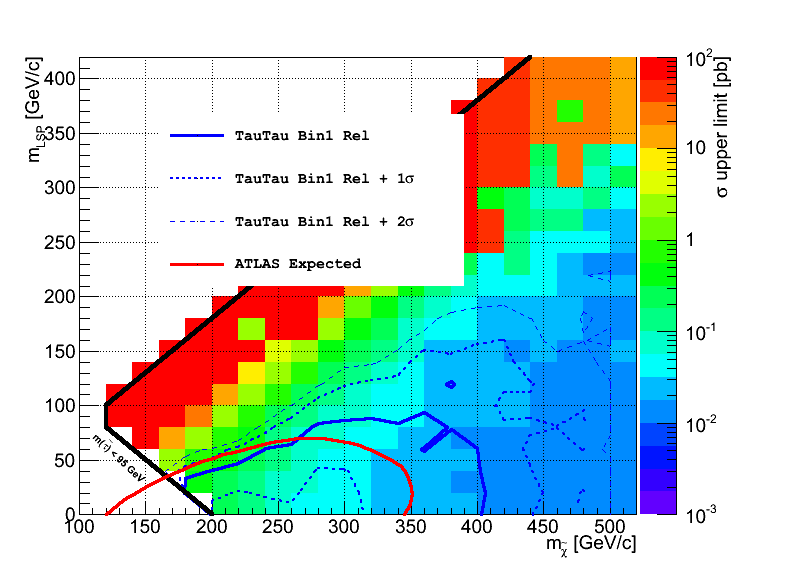
\includegraphics[width=0.49\textwidth,keepaspectratio=true]{StatisticsFig/NewFigs/TauTau_Bin1Rel.png}
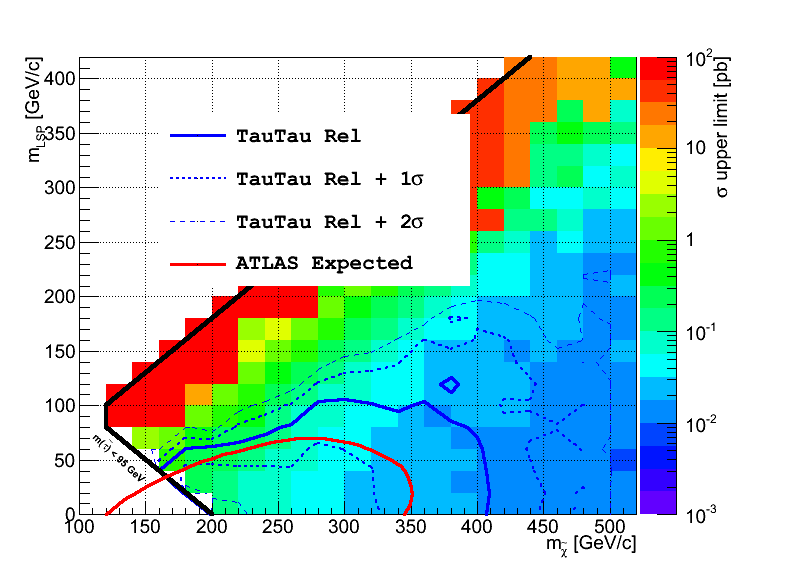
\includegraphics[width=0.49\textwidth,keepaspectratio=true]{StatisticsFig/NewFigs/TauTau_Bin1Rel_Bin2.png}
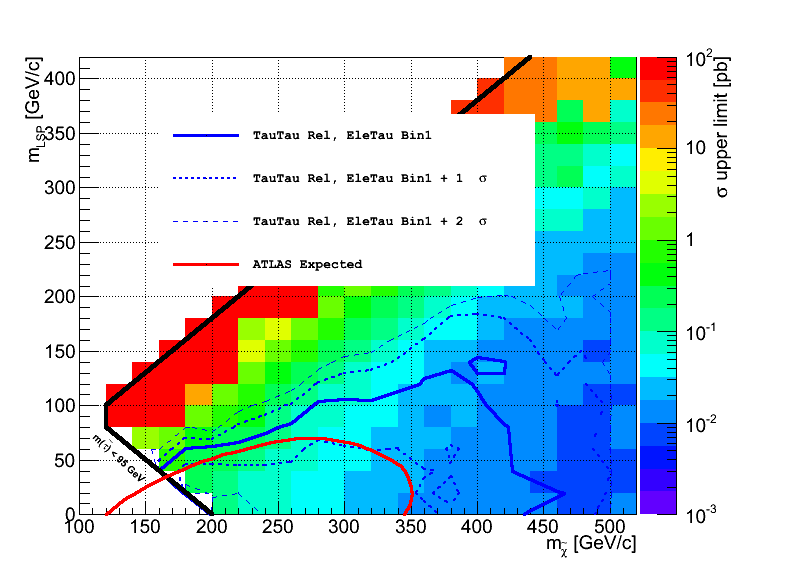
\includegraphics[width=0.49\textwidth,keepaspectratio=true]{StatisticsFig/NewFigs/TauTau_EleTauBin1.png}
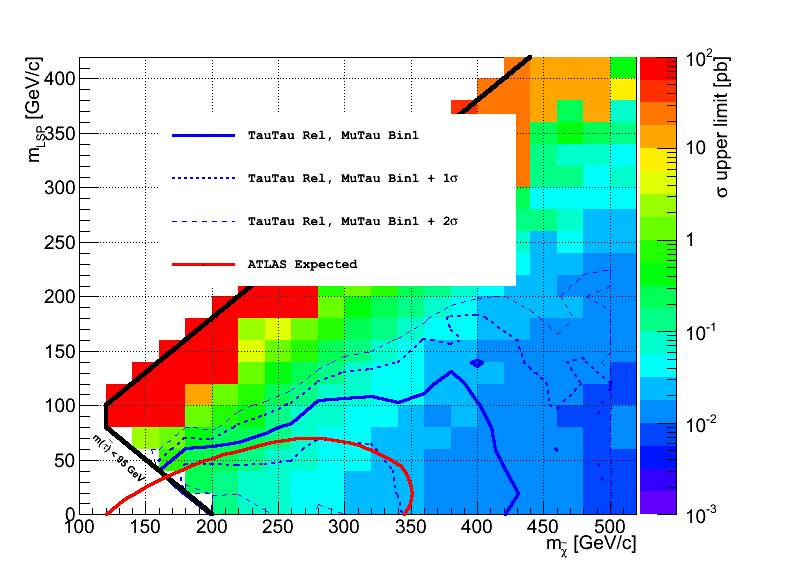
\includegraphics[width=0.49\textwidth,keepaspectratio=true]{StatisticsFig/NewFigs/TauTau_MuTauBin1.png}
\caption{These figures show the impact of each bin on the final combination. 
The top panels are related to the $\tau_{had}-\tau_{had}~$ channel including the bin 1 alone (left) and combination of bins 1 and 2 (right).
The bottom ones show the expected exclusion limit when $e-\tau_{had}~$ (left) and $\mu-\tau_{had}~$ (right) channels are included in the $\tau_{had}-\tau_{had}~$ channel.
}
\label{fig:limit_bins}
\end{figure}
\end{linenomath}
%%%%%%%%%%


Figure \ref{fig:limit_final} shows the expected upper limit on the cross section of the chargino pair production in terms of Simplified Models. 
The signal rates for each bin are 0.5420, 1.7200, 1.5800 and 0.7680, 
while overall background rates are 3.01, 1.5, 2.7 and 1.06 respectively.
However, backgrounds are taken into account in two categories, including Monte-Carlo-Driven (MCD), Data-Driven (DD).
Due to the method of background estimation in the $\tau_{had}-\tau_{had}~$ channel, bins 1 and 2 have a more category called W-jets (W).    
MCD backgrounds are feed to the package as a Gamma distribution with the corresponding statistical weights for each bin.
Furthermore, 25\% systematic uncertainity on MCD backgrounds is also considered.
All systematics are taken through LogNormal distributions.
Systematic uncertainities for each bin of DD backgrounds are 15\%, 11\%, 50\% and 69\% respectively. (numbers must be corrected)  
W backgronds have 37\% and 45\% systematic uncertainity for the first and second bins respectively.
And finally, 20\% systematic uncertainity on signal yields is considered. 
Calculation of the expected exclusion limit shows that the research has potential to exclude 
%excludes 
a sizable region of the phase space, surrounded by the lines of $m_{\PSGcpmDo} = 500\GeV$ and $m_{\PSGczDo} = 150\GeV$ with an integrated luminosity of $19.6\,\fbinv$.
The Red curve represents the expected reach by ATLAS %\cite{cutandcountAN}
 search. As the figure shows our analysis (the blue solid curve) improves the ATLAS result in the $m_{\PSGcpmDo}-m_{\PSGczDo}$ plane.

%%%%%%%%%%
\begin{linenomath}
\begin{figure}[h]
\centering
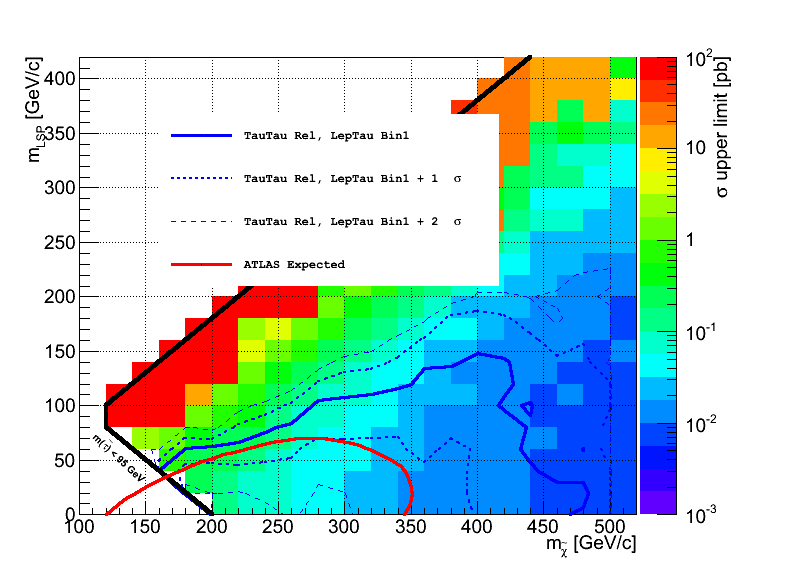
\includegraphics[width=0.7\textwidth,keepaspectratio=true]{StatisticsFig/NewFigs/Final_4BinRel.png}
\caption{Expected exclusion power in terms of Simplified Models %(T2tt-topology) 
with an integrated luminosity of $20\,\fbinv$. Backgrounds are predicted using Monte-Carlo simulations and a rough estimate of systematic uncertainties equal 
$10\%$ is taken into account.}
\label{fig:limit_final}
\end{figure}
\end{linenomath}
%%%%%%%%%%


%\rule{\textwidth}{1pt}

%In this study, we analyze data in 8 different bins (multi-bin analysis) to utilize more information from 
%the observed and the predicted distributions.
%bins' contents of the observations and the predictions.
%The bins are defined in reconstructed top quark multiplicity, zero or more. In addition, events are categorized based on the $\mttwo$ values: $125\GeV \leq \mttwo < 150\GeV,\; 150\GeV \leq \mttwo < 200\GeV,\; 200\GeV \leq \mttwo < 250\GeV,\; 250\GeV \leq \mttwo < \infty$.
%These bins are determined, for an event, based on whether the event contents reconstructed top quarks or not (2 bins) times which bin of $\mttwo$ is occupied by the event (4 bins of $125\GeV \leq \mttwo < 150\GeV,\; 150\GeV \leq \mttwo < 200\GeV,\; 200\GeV \leq \mttwo < 250\GeV,\; 250\GeV \leq \mttwo < \infty$). 

%To investigate the exclusion power of our research, we study the topology of direct stop pair production  in Simplified Models \cite{alves:sms}, with $\tilde{t}\to \PSGczDo t$ (T2tt). 
%Calculation of the expected exclusion limit shows that  
%the research has potential to exclude 
%excludes 
%a sizable region of the phase space, surrounded by the lines of $m_{\tilde{t}} = 600\GeV$ and $m_{\PSGczDo} = 175\GeV$ with an integrated luminosity of $19.6\,\fbinv$.



%Figure \ref{fig:limit_20inf} shows the expected upper limit on the cross section of the stop pair production in terms of Simplified Models. 
%Furthermore, the figure shows the expected exclusion power considering 
%$40\%$ systematic uncertainties on signal and background rates which are predicted using Monte-Carlo simulations. The black 
%dashed curve represents the expected reach by the common Cut$\&$Count \cite{cutandcountAN} search using $\MET$ trigger. 
%As the figure shows our analysis (the blue solid curve) can be comparable with other analyses and   
%it has the potential to be complementary to other analyses in some regions of the phase space.  



%%%%%%%%%%
%\begin{linenomath}
%\begin{figure}[h]
%\centering
%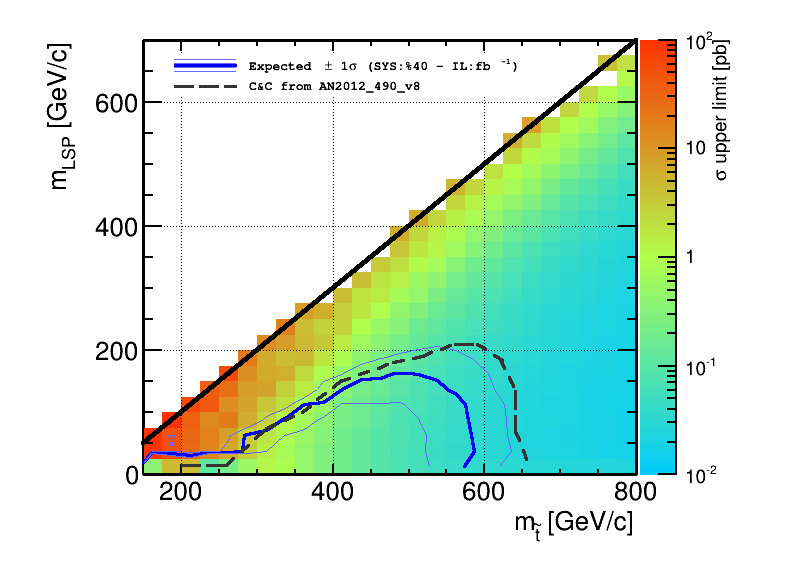
\includegraphics[width=0.9\textwidth,keepaspectratio=true]{StatisticsFig/Exc_131030_196ifb.png}
%\caption{Expected exclusion power in terms of Simplified Models (T2tt-topology) with an integrated luminosity of $20\,\fbinv$. Backgrounds are predicted using Monte-Carlo simulations and a rough estimate of systematic uncertainties equal 
%$40\%$ is taken into account.}
%\label{fig:limit_20inf}
%\end{figure}
%\end{linenomath}
%%%%%%%%%%


%%%%%%%%%%
%\begin{linenomath}
%\begin{figure}[h]
%\centering
%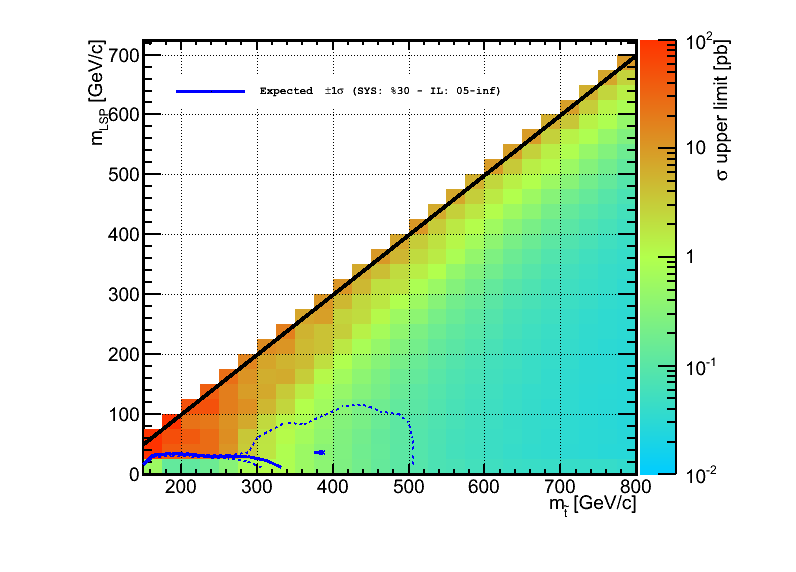
\includegraphics[width=0.7\textwidth,keepaspectratio=true]{StatisticsFig/limit_30sys_05inf_20130625.png}
%\caption{}
%\label{fig:limit_05inf}
%\end{figure}
%\end{linenomath}
%%%%%%%%%%

%%%%%%%%%%
%\begin{linenomath}
%\begin{figure}[h]
%\centering
%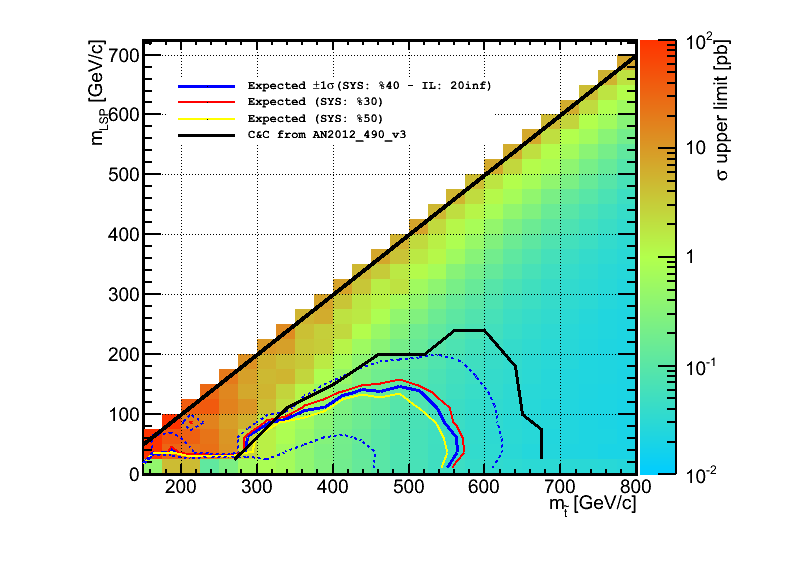
\includegraphics[width=0.7\textwidth,keepaspectratio=true]{StatisticsFig/limit_304050sys_20inf_20130625.png}
%\caption{}
%\label{fig:limit_20inf}
%\end{figure}
%\end{linenomath}
%%%%%%%%%%


\section{Information to test the new models}
\label{sect:model}
In the previous sections, a simplified SUSY model was used to optimize the selections and interpret the results. 
Here, the main efficiencies and weights are reported versus the generated values, that can be used to examine 
the new models approximately in a Monte Carlo generator-level study. 
The number of the remaining signal events and its uncertainty which can be evaluated by a generator-level study 
should be combined statistically with the results in Table \ref{tbl:yieldSysSummary} to find the upper limit 
on the number of the signal events
and decide if a model is excluded or still allowed in the shadow of the analysis presented in the paper.

Efficiencies are provided against the keinematic properties (e.g., \pt) of visible $\tau$'s at generator level. The visible $\tau$ (\visTau), if it decays leptonically, is defined as the 4-vector of the lepton. In hadronic decays, the difference between the 4-vector of $\tau$ and its neutrino is attributed to the visible $\tau$. %It is, hereafter, referred to as \visTau.
Table \ref{tbl:EffTauLep}
\begin{table}[!htb]
\begin{center}
\caption{Weights to select a lepton or \Tau in different channels. $\Tau^1$ and $\Tau^2$ stand for leading and next-to-leading \Tau in the \tauTau channel.}
\begin{tabular}{|c|c|c|c|c|c|}
\hline\hline
\pt(\visTau) (\GeV)  & e for $e\Tau$ & $\mu$ for $\mu\Tau$  & \Tau for $\ell\Tau$    &  $\Tau^1$ for \tauTau & $\Tau^2$ for \tauTau\\
\hline\hline
0-10                      &    0.15       &    0.05              &         0.001          &       0.0             & 0.52 \\\hline
10-20                     &    0.14       &    0.72              &         0.004          &       0.0             & 0.54\\\hline
20-30                     &    0.27       &    0.80              &         0.11           &       0.0             & 0.56\\\hline
30-40                     &    0.68       &    0.85              &         0.22           &       0.0             & 0.55\\\hline
40-60                     &    0.75       &    0.87              &         0.24           &       0.02            & 0.61\\\hline
60-80                     &    0.80       &    0.88              &         0.25           &       0.08            & 0.69\\\hline
80-120                    &    0.83       &    0.89              &         0.27           &       0.12            & 0.70\\\hline
120-160                   &    0.85       &    0.90              &         0.28           &       0.15            & 0.70\\\hline
160-200                   &    0.87       &    0.91              &         0.28           &       0.16            & 0.71\\\hline
$>$ 200                   &    0.89       &    0.92              &         0.29           &       0.17            & 0.71\\\hline
\hline
\end{tabular}
\label{tbl:EffTauLep}
\end{center}
\end{table}
shows the weights of selecting a lepton or \Tau for different channels versus the \pt(\visTau). The \visMET variable is defined as the magnitude of the negative vector sum of \visTau pairs in the transverse plane. 
Table \ref{tbl:EffMet}
\begin{table}[!htb]
\begin{center}
\caption{Efficiency to pass the \MPT  requirement in different channels versus the \visMET.}
\begin{tabular}{|c|c|}
\hline\hline
\visMET  (\GeV)        & all channels\\
\hline\hline
0-10                   &    0.52 \\\hline
10-20                  &    0.57 \\\hline
20-30                  &    0.68 \\\hline
30-40                  &    0.79 \\\hline
40-50                  &    0.87 \\\hline
50-60                  &    0.93 \\\hline
60-70                  &    0.95 \\\hline
70-80                  &    0.97 \\\hline
80-90                  &    0.98 \\\hline
90-100                 &    0.98 \\\hline
100-120                &    0.99 \\\hline
120-140                &    0.99 \\\hline
140-160                &    0.99 \\\hline
160-200                &    1.0  \\\hline
$>$ 200                &    1.0  \\\hline
\hline
\end{tabular}
\label{tbl:EffMet}
\end{center}
\end{table}
shows the efficiency in different channels to pass the \MPT $>$ 30 \GeV as a function of the \visMET. 
%The mass of the system of the selected pair is used to parametrize 
%the efficiency to pass the cuts on the reconstructed invariant mass. 
Table \ref{tbl:EffMass}
\begin{table}[!htb]
\begin{center}
\caption{Efficiency to pass the invariant mass requirements in different channels versus the visible mass.}
\begin{tabular}{|c|c|c|}
\hline\hline
visible mass (\GeV)  & $\ell\Tau$  &  \tauTau \\
\hline\hline
0-5                  &    0.00     &   0.00   \\\hline
5-10                 &    0.26     &   0.25   \\\hline
10-15                &    0.65     &   0.60  \\\hline
15-20                &    0.96     &   0.90  \\\hline
20-25                &    0.99     &   0.94   \\\hline
25-30                &    0.99     &   0.98   \\\hline
30-35                &    0.99     &   1.00   \\\hline
35-40                &    0.98     &   1.00   \\\hline
40-45                &    0.83     &   0.99   \\\hline
45-50                &    0.15     &   0.95   \\\hline
50-55                &    0.03     &   0.68   \\\hline
55-60                &    0.02     &   0.18   \\\hline
60-65                &    0.02     &   0.06   \\\hline
65-70                &    0.04     &   0.03   \\\hline
70-75                &    0.22     &   0.05   \\\hline
75-80                &    0.78     &   0.15   \\\hline
80-85                &    0.92     &   0.41   \\\hline
85-90                &    0.95     &   0.79   \\\hline
90-95                &    0.97     &   0.93   \\\hline
95-100               &    0.99     &   0.96   \\\hline
100-105              &    1.00     &   0.98   \\\hline
105-110              &    1.00     &   0.99   \\\hline
110-115              &    1.00     &   0.99   \\\hline
$>$ 115              &    1.00     &   1.00   \\\hline
\hline
\end{tabular}
\label{tbl:EffMass}
\end{center}
\end{table}
shows the efficiency in different channels to pass the requirement of the reconstructed invariant mass versus the invariant mass of  
\visTau pair (visible mass). The requirements
on the invariant mass of the reconstructed pair are ($>$ 15 \GeV) and ($<$ 45 or $>$ 75 \GeV) for the $\ell\Tau$ channels 
and ($<$ 55 or $>$ 85 \GeV) for the \tauTau channel. 
The 4-vector of the particles of \visTau pair and \visMET are used to calculate the visible \mttwo. The efficiency to pass the (\mttwo $>$ 90 \GeV) requirement in $\ell\Tau$ and \tauTau \binone is shown in Table \ref{tbl:EffMT2}. 
\begin{table}[!htb]
\begin{center}
\caption{Efficiency to pass the  \mttwo $>$ 90 \GeV requirement in different channels versus the visible \mttwo.}
\begin{tabular}{|c|c|c|}
\hline\hline
visible \mttwo (\GeV)    & $\ell\Tau$  &  \tauTau \binone \\
\hline\hline
0-20                     &    0.00     &   0.00  \\\hline
20-40                    &    0.003    &   0.01  \\\hline
40-50                    &    0.01     &   0.02  \\\hline
50-60                    &    0.02     &   0.04  \\\hline
60-70                    &    0.05     &   0.08  \\\hline
70-80                    &    0.14     &   0.19  \\\hline
80-90                    &    0.35     &   0.45  \\\hline
90-100                   &    0.65     &   0.73  \\\hline
100-110                  &    0.82     &   0.88  \\\hline
110-120                  &    0.89     &   0.94  \\\hline
120-130                  &    0.93     &   0.97  \\\hline
130-140                  &    0.95     &   0.98  \\\hline
140-160                  &    0.96     &   0.99  \\\hline
160-180                  &    0.97     &   0.99  \\\hline
180-200                  &    0.97     &   1.00  \\\hline
$>$ 200                  &    0.97     &   1.00  \\\hline
\hline
\end{tabular}
\label{tbl:EffMT2}
\end{center}
\end{table}
In the $\ell\Tau$ channels, to calculate the visible \tauMT, the 4-vector of the visible \Tau and \visMET are used. Table \ref{tbl:EffTauMT}
\begin{table}[!htb]
\begin{center}
\caption{Efficiency to pass the  \tauMT requirement in $\ell\Tau$ channels versus the visible \tauMT.}
\begin{tabular}{|c|c|}
\hline\hline
visible \tauMT (\GeV)  & $\ell\Tau$ \\
\hline\hline
0-50                     &   0.35   \\\hline
50-100                   &   0.1   \\\hline
100-125                  &   0.05   \\\hline
125-150                  &   0.07   \\\hline
150-170                  &   0.14   \\\hline
170-190                  &   0.32   \\\hline
190-200                  &   0.55   \\\hline
200-210                  &   0.68   \\\hline
210-230                  &   0.83   \\\hline
230-250                  &   0.91   \\\hline
250-275                  &   0.95   \\\hline
275-300                  &   0.97   \\\hline
$>$ 300                  &   0.99   \\\hline
\hline
\end{tabular}
\label{tbl:EffTauMT}
\end{center}
\end{table}
shows the efficiency in the $\ell\Tau$ channels to pass the   \tauMT $>$ 200 \GeV requirement versus the generated \tauMT.


In the \tauTau \bintwo, the reconstructed \mttwo is constrained between 40 and 90 \GeV. Table \ref{tbl:EffMT2SR2}
\begin{table}[!htb]
\begin{center}
\caption{Efficiency to pass the \mttwo requirement in \tauTau \bintwo versus the visible \mttwo.}
\begin{tabular}{|c|c|}
\hline\hline
generated \mttwo (\GeV)  &  \tauTau \bintwo \\
\hline\hline
0-10                     &   0.007   \\\hline
10-20                    &   0.10    \\\hline
20-30                    &   0.26    \\\hline
30-40                    &   0.57    \\\hline
40-50                    &   0.85    \\\hline
50-60                    &   0.93    \\\hline
60-70                    &   0.92    \\\hline
70-80                    &   0.82    \\\hline
80-90                    &   0.56    \\\hline
90-100                   &   0.27    \\\hline
100-110                  &   0.12    \\\hline
110-120                  &   0.06    \\\hline
120-130                  &   0.03    \\\hline
130-140                  &   0.02    \\\hline
$>$ 140                  &   0.01    \\\hline
\hline
\end{tabular}
\label{tbl:EffMT2SR2}
\end{center}
\end{table}
shows the efficiency in \tauTau \bintwo to pass the 40 $<$ \mttwo $<$ 90 \GeV requirement versus the visible \mttwo. 
The last selection in this channel is
the requirement on \SumMT which is calculated using the 4-vector of two \visTau and \visMET. Table \ref{tbl:EffSumMT} 
\begin{table}[!htb]
\begin{center}
\caption{Efficiency to pass the \SumMT requirement in \tauTau \bintwo versus the visible \SumMT.}
\begin{tabular}{|c|c|c|}
\hline\hline
visible \SumMT (\GeV)  &  \tauTau \bintwo\\
\hline\hline
$<$ 60                 &   0.00  \\\hline
60-80                  &   0.84  \\\hline
80-100                 &   0.68  \\\hline
100-120                &   0.45  \\\hline
120-140                &   0.29  \\\hline
140-160                &   0.22  \\\hline
160-180                &   0.18  \\\hline
180-200                &   0.22  \\\hline
200-210                &   0.28  \\\hline
210-220                &   0.34  \\\hline
220-230                &   0.41  \\\hline
230-240                &   0.49  \\\hline
240-250                &   0.59  \\\hline
250-260                &   0.63  \\\hline
260-270                &   0.70  \\\hline
270-280                &   0.76  \\\hline
280-290                &   0.78  \\\hline
290-300                &   0.83  \\\hline
300-320                &   0.87  \\\hline
320-340                &   0.88  \\\hline
340-360                &   0.91  \\\hline
360-380                &   0.92  \\\hline
380-400                &   0.92  \\\hline
400-420                &   0.93  \\\hline
420-440                &   0.93  \\\hline
440-460                &   0.88  \\\hline
460-480                &   0.89  \\\hline
480-500                &   0.93  \\\hline
$>$ 500                &   0.81  \\\hline
\hline
\end{tabular}
\label{tbl:EffSumMT}
\end{center}
\end{table}
shows the efficiency in \tauTau \bintwo to pass the \SumMT $>$ 250 \GeV requirement versus the generated \SumMT.

To use these efficiencies, one needs to multiply the values one after another and combine the final value with the values reported in Table \ref{tbl:yieldSysSummary}  statistically, to decide if a signal point is not still excluded. In the generator level, only a pair of $\ell\Tau$ or \tauTau is selected and no other selection is applied.

To take into account the inefficiencies and misidentifications for charge reconstruction of the objects, b-tagging of the jets, identification of the extra leptons 
and the minimum angle between the jets and \MPT in the transverse plane, the extra factors shown in Table \ref{tbl:EffSF} need to be applied.
\begin{table}[!htb] 
\begin{center}
\caption{Extra factors to take into account the inefficiencies and misidentifications introduced by detector simulation and reconstruction.}
\begin{tabular}{|c|c|c|c|}
\hline\hline
       &   $\ell\Tau$  &  \tauTau \binone & \tauTau \bintwo\\
\hline\hline
factor &       0.75    &       0.48       &    0.56 \\\hline
\hline
\end{tabular}
\label{tbl:EffSF}
\end{center}
\end{table}

The efficiencies were used to reproduce the yields in the SMS plane. The results were in agreement with the yields from the full chain of 
simulation and reconstruction within ~10\%.


\section{Conclusion}
\label{sect:conclusion}
A search for SUSY in $\tau\tau$ final state is presented. The $\tau$ pair is produced in a cascade from the production of the \PSGcpDo pair.
Different channels and search bins are introduced to increase the sensitivity to different parts of the phase space. 
Backgrounds and their systematics are discussed in details. The expected exclusion limits are also presented for different combination of the 
channels.

\section{Acknowledgments}
This analysis benefits highly from the computing resources of T2 at UCSD and codes developed in ETHZurich. 
We appreciate their help and generosity.
The authors would like to thank the previous and current conveners of the SUSY and SUSY-TBT working group, Frank Wuerthwein, Keith Ulmer, Filip Moortgat, Joshua Thompson, Pieter Everaerts and Boris Mangano for their help and support. 
The authors would like to thank the management and staff of the school of particles 
and accelerators of IPM, especially Prof. Arfaei for their help and support. 
We had several discussions with our colleagues at LIP, Pedram Bargassa, Michele Gallinaro and Cristovao Beirao Da Cruz E Silva. 
We would like to thank them for their helps and suggestions.
Thanks to all of the members of
the CMS collaboration for their outstanding results discussed partly here.

% >> acknowledgments (for journal papers)
% Please include the latest version from https://twiki.cern.ch/twiki/bin/viewauth/CMS/Internal/PubAcknow.
%\begin{acknowledgments}...ack-text...\end{acknowledgments}
% This will normally be updated with the text available at the time of submission,
% so please add a comment if it has been modified. Such modifications need to be
% approved.
%

%\begin{acknowledgments}
\section*{Acknowledgements}
\hyphenation{Bundes-ministerium Forschungs-gemeinschaft Forschungs-zentren} We congratulate our colleagues in the CERN accelerator departments for the excellent performance of the LHC and thank the technical and administrative staffs at CERN and at other CMS institutes for their contributions to the success of the CMS effort. In addition, we gratefully acknowledge the computing centers and personnel of the Worldwide LHC Computing Grid for delivering so effectively the computing infrastructure essential to our analyses. Finally, we acknowledge the enduring support for the construction and operation of the LHC and the CMS detector provided by the following funding agencies: the Austrian Federal Ministry of Science, Research and Economy and the Austrian Science Fund; the Belgian Fonds de la Recherche Scientifique, and Fonds voor Wetenschappelijk Onderzoek; the Brazilian Funding Agencies (CNPq, CAPES, FAPERJ, and FAPESP); the Bulgarian Ministry of Education and Science; CERN; the Chinese Academy of Sciences, Ministry of Science and Technology, and National Natural Science Foundation of China; the Colombian Funding Agency (COLCIENCIAS); the Croatian Ministry of Science, Education and Sport, and the Croatian Science Foundation; the Research Promotion Foundation, Cyprus; the Ministry of Education and Research, Estonian Research Council via IUT23-4 and IUT23-6 and European Regional Development Fund, Estonia; the Academy of Finland, Finnish Ministry of Education and Culture, and Helsinki Institute of Physics; the Institut National de Physique Nucl\'eaire et de Physique des Particules~/~CNRS, and Commissariat \`a l'\'Energie Atomique et aux \'Energies Alternatives~/~CEA, France; the Bundesministerium f\"ur Bildung und Forschung, Deutsche Forschungsgemeinschaft, and Helmholtz-Gemeinschaft Deutscher Forschungszentren, Germany; the General Secretariat for Research and Technology, Greece; the National Scientific Research Foundation, and National Innovation Office, Hungary; the Department of Atomic Energy and the Department of Science and Technology, India; the Institute for Studies in Theoretical Physics and Mathematics, Iran; the Science Foundation, Ireland; the Istituto Nazionale di Fisica Nucleare, Italy; the Ministry of Science, ICT and Future Planning, and National Research Foundation (NRF), Republic of Korea; the Lithuanian Academy of Sciences; the Ministry of Education, and University of Malaya (Malaysia); the Mexican Funding Agencies (CINVESTAV, CONACYT, SEP, and UASLP-FAI); the Ministry of Business, Innovation and Employment, New Zealand; the Pakistan Atomic Energy Commission; the Ministry of Science and Higher Education and the National Science Centre, Poland; the Funda\c{c}\~ao para a Ci\^encia e a Tecnologia, Portugal; JINR, Dubna; the Ministry of Education and Science of the Russian Federation, the Federal Agency of Atomic Energy of the Russian Federation, Russian Academy of Sciences, and the Russian Foundation for Basic Research; the Ministry of Education, Science and Technological Development of Serbia; the Secretar\'{\i}a de Estado de Investigaci\'on, Desarrollo e Innovaci\'on and Programa Consolider-Ingenio 2010, Spain; the Swiss Funding Agencies (ETH Board, ETH Zurich, PSI, SNF, UniZH, Canton Zurich, and SER); the Ministry of Science and Technology, Taipei; the Thailand Center of Excellence in Physics, the Institute for the Promotion of Teaching Science and Technology of Thailand, Special Task Force for Activating Research and the National Science and Technology Development Agency of Thailand; the Scientific and Technical Research Council of Turkey, and Turkish Atomic Energy Authority; the National Academy of Sciences of Ukraine, and State Fund for Fundamental Researches, Ukraine; the Science and Technology Facilities Council, UK; the US Department of Energy, and the US National Science Foundation.

Individuals have received support from the Marie-Curie programme and the European Research Council and EPLANET (European Union); the Leventis Foundation; the A. P. Sloan Foundation; the Alexander von Humboldt Foundation; the Belgian Federal Science Policy Office; the Fonds pour la Formation \`a la Recherche dans l'Industrie et dans l'Agriculture (FRIA-Belgium); the Agentschap voor Innovatie door Wetenschap en Technologie (IWT-Belgium); the Ministry of Education, Youth and Sports (MEYS) of the Czech Republic; the Council of Science and Industrial Research, India; the HOMING PLUS programme of Foundation for Polish Science, cofinanced from European Union, Regional Development Fund; the Compagnia di San Paolo (Torino); the Consorzio per la Fisica (Trieste); MIUR project 20108T4XTM (Italy); the Thalis and Aristeia programmes cofinanced by EU-ESF and the Greek NSRF; and the National Priorities Research Program by Qatar National Research Fund. 
%\end{acknowledgments}
%% **DO NOT REMOVE BIBLIOGRAPHY**
\bibliography{auto_generated}   % will be created by the tdr script.

%%% DO NOT ADD \end{document}!

